%! TEX root = main.tex
\documentclass{article}
\usepackage[utf8]{inputenc}
\usepackage[spanish,mexico]{babel}
\usepackage{graphicx}
\usepackage{xcolor}
\usepackage{amsmath,amssymb}
\usepackage{booktabs}
\usepackage{tabularx}
\usepackage{adjustbox}
\usepackage{hyperref}
\usepackage{float}
\usepackage{tikz}
\usetikzlibrary{shapes.geometric, arrows.meta, positioning, calc, shadows, fit, backgrounds}
\usepackage{multicol}
\usepackage{geometry}

\geometry{
  a4paper,
  left=1.5cm,
  right=1.5cm,
  top=1.8cm,
  bottom=2.0cm
}

\hypersetup{
    colorlinks=true,
    linkcolor=blue!70!black,
    citecolor=blue!70!black,
    urlcolor=blue!70!black
}

% ESTILOS TIKZ PARA DIAGRAMAS DE FLUJO E INFOGRAFÍAS
\tikzset{
    startstop/.style={
        rectangle, rounded corners=12pt, minimum width=2.8cm, minimum height=0.9cm,
        align=center, draw=black!80, fill=blue!15, drop shadow, font=\small\bfseries
    },
    process/.style={
        rectangle, rounded corners=4pt, minimum width=3.2cm, minimum height=1.0cm,
        align=center, text width=3.2cm, draw=blue!70!black, fill=blue!5, drop shadow, font=\footnotesize
    },
    process_green/.style={
        rectangle, rounded corners=4pt, minimum width=3.2cm, minimum height=1.0cm,
        align=center, text width=3.2cm, draw=green!60!black, fill=green!5, drop shadow, font=\footnotesize
    },
    process_orange/.style={
        rectangle, rounded corners=4pt, minimum width=3.2cm, minimum height=1.0cm,
        align=center, text width=3.2cm, draw=orange!80!black, fill=orange!8, drop shadow, font=\footnotesize
    },
    decision/.style={
        diamond, aspect=2, minimum width=2.8cm, minimum height=1.0cm,
        align=center, text width=2.6cm, draw=purple!80!black, fill=purple!10, drop shadow, font=\footnotesize\bfseries
    },
    arrow/.style={
        thick, -{Latex[length=2.5mm, width=1.8mm]}, draw=gray!80!black
    },
    arrow_green/.style={
        thick, -{Latex[length=2.5mm, width=1.8mm]}, draw=green!60!black
    },
    arrow_blue/.style={
        thick, -{Latex[length=2.5mm, width=1.8mm]}, draw=blue!70!black
    },
    neuron_node/.style={
        circle, draw=blue!80!black, fill=blue!10, minimum size=0.9cm, align=center, font=\small\bfseries
    },
    sum_node/.style={
        circle, draw=orange!80!black, fill=orange!20, minimum size=1.1cm, align=center, font=\large\bfseries
    },
    func_node/.style={
        rectangle, rounded corners=3pt, draw=teal!80!black, fill=teal!15, minimum size=1.0cm, align=center, font=\small\bfseries
    }
}

\begin{document}

% ENCABEZADO INSTITUCIONAL - PLANTILLA MCIC
\colorbox{white!10!}{
    \begin{minipage}[t]{0.165 \textwidth}
       \begin{flushright}
        
\includegraphics[width=0.85in]{EscudoUD.png}
       \end{flushright}
    \end{minipage}
    \begin{minipage}[H]{0.62 \textwidth}
        \begin{center}
            {\large \textsc{Universidad Distrital Francisco José de Caldas}}
            \vspace{0.4cm}
            \\
            { \huge \textbf{Taller 1: Perceptrón Simple y Adaline}}
            \\
            \vspace{0.25cm}
            \small{\textbf{Maestría en Ciencias de la Información y las Comunicaciones (MCIC)}}\\
            \textbf{Inteligencia Computacional Aplicada} -- \textit{Docente: Cesar Andrey Perdomo Charry}
            \begin{center}
                \small \textbf{Estudiante:} Juan Felipe Rodríguez Galindo \quad | \quad \textbf{Código:} 20261595004
            \end{center}
        \end{center}
        \vspace{0.05cm}
    \end{minipage}
    \begin{minipage}[t]{0.165\textwidth}
        \raggedright
        
\includegraphics[width=1.15in]{LogoMCIC.png}
    \end{minipage}
}

\begin{tikzpicture}
    \draw[thick] (-0.5,0)--(17.5,0);
\end{tikzpicture}

\vspace{0.3cm}

\begin{abstract}
En el presente informe se describe el desarrollo, implementación y análisis comparativo de dos de los modelos de la computación neuronal: el \textbf{Perceptrón Simple} de Rosenblatt y la red \textbf{Adaline} (\textit{Adaptive Linear Neuron}) de Widrow y Hoff. Las arquitecturas fueron programadas desde cero en Python, estructurando las ejecuciones en un cuaderno interactivo de Jupyter. Se evalúa el comportamiento de ambos modelos ante compuertas lógicas canónicas ($\text{AND}$ y $\text{OR}$ de 2, 3 y 4 entradas) y ante dos conjuntos de datos multidimensionales: el dataset \textbf{Iris} (clasificación linealmente separable de \textit{Iris Setosa}) y el dataset \textbf{Banknote Authentication} (1372 instancias, 4 atributos continuos). Se analizan tres reglas de corrección de pesos para el perceptrón, el impacto del factor relativo de aprendizaje $\alpha$, la convergencia del error cuadrático medio (MSE) en Adaline, y la estabilidad del aprendizaje bajo particiones de entrenamiento y prueba de 60-40, 70-30, 80-20 y 90-10 según la metodología de muestreo de \texttt{Dataset\_train\_test.mlx}.
\end{abstract}

\vspace{0.2cm}

\section{Introducción y Marco Teórico}
El desarrollo histórico de las redes neuronales artificiales parte de la concepción de unidades de procesamiento capaces de ajustar sus parámetros internos mediante retroalimentación basada en errores. Dos hitos determinantes en esta evolución son el Perceptrón Simple (1958) y el modelo Adaline (1960). A pesar de compartir una topología elemental de una sola capa y una sola neurona, sus fundamentos matemáticos y dinámicas de optimización difieren sustancialmente.

\subsection{Modelo del Perceptrón Simple}
El perceptrón calcula una combinación lineal ponderada de las entradas aumentadas con una entrada constante $x_0 = 1$ asociada al sesgo o \textit{bias} $w_0$:
\begin{equation}
z = W^T X = w_0 + \sum_{i=1}^n w_i x_i
\end{equation}
La señal resultante pasa a través de una función de activación escalón unitario (\textit{Step Function}):
\begin{equation}
Y(x) = \begin{cases} 
1 & \text{si } z \ge \theta \\ 
0 & \text{si } z < \theta 
\end{cases}
\end{equation}
donde $\theta$ representa el umbral de activación del modelo. La actualización de los pesos se realiza de acuerdo con:
\begin{equation}
W_i^* = W_i + \Delta W_i
\end{equation}

En el presente taller se evalúan las tres reglas de actualización especificadas:
\begin{itemize}
    \item \textbf{Regla 1:} $\Delta W_i = d(x) \cdot X_i$. Ajuste aditivo dependiente únicamente del valor deseado $d(x)$ y de la entrada $X_i$.
    \item \textbf{Regla 2:} $\Delta W_i = [d(x) - Y(x)] \cdot X_i$. Regla clásica de corrección por error discreto con factor unitario ($\alpha = 1$).
    \item \textbf{Regla 3:} $\Delta W_i = \alpha \cdot [d(x) - Y(x)] \cdot X_i$. Regla estándar del perceptrón modulada por la tasa de aprendizaje $\alpha > 0$.
\end{itemize}

\begin{figure}[H]
    \centering
    \begin{minipage}[b]{0.48\textwidth}
        \centering
        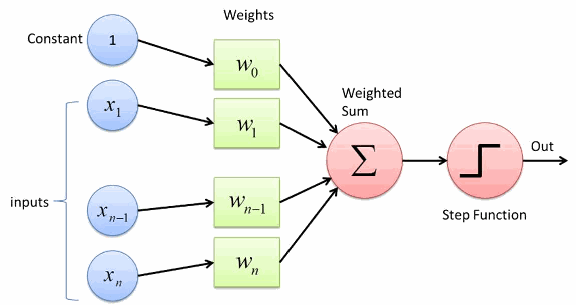
\includegraphics[width=\textwidth]{figuras/modelo_perceptron.png}
        \caption{Modelo esquemático del Perceptrón Simple.}
        \label{fig:modelo_perceptron}
    \end{minipage}
    \hfill
    \begin{minipage}[b]{0.48\textwidth}
        \centering
        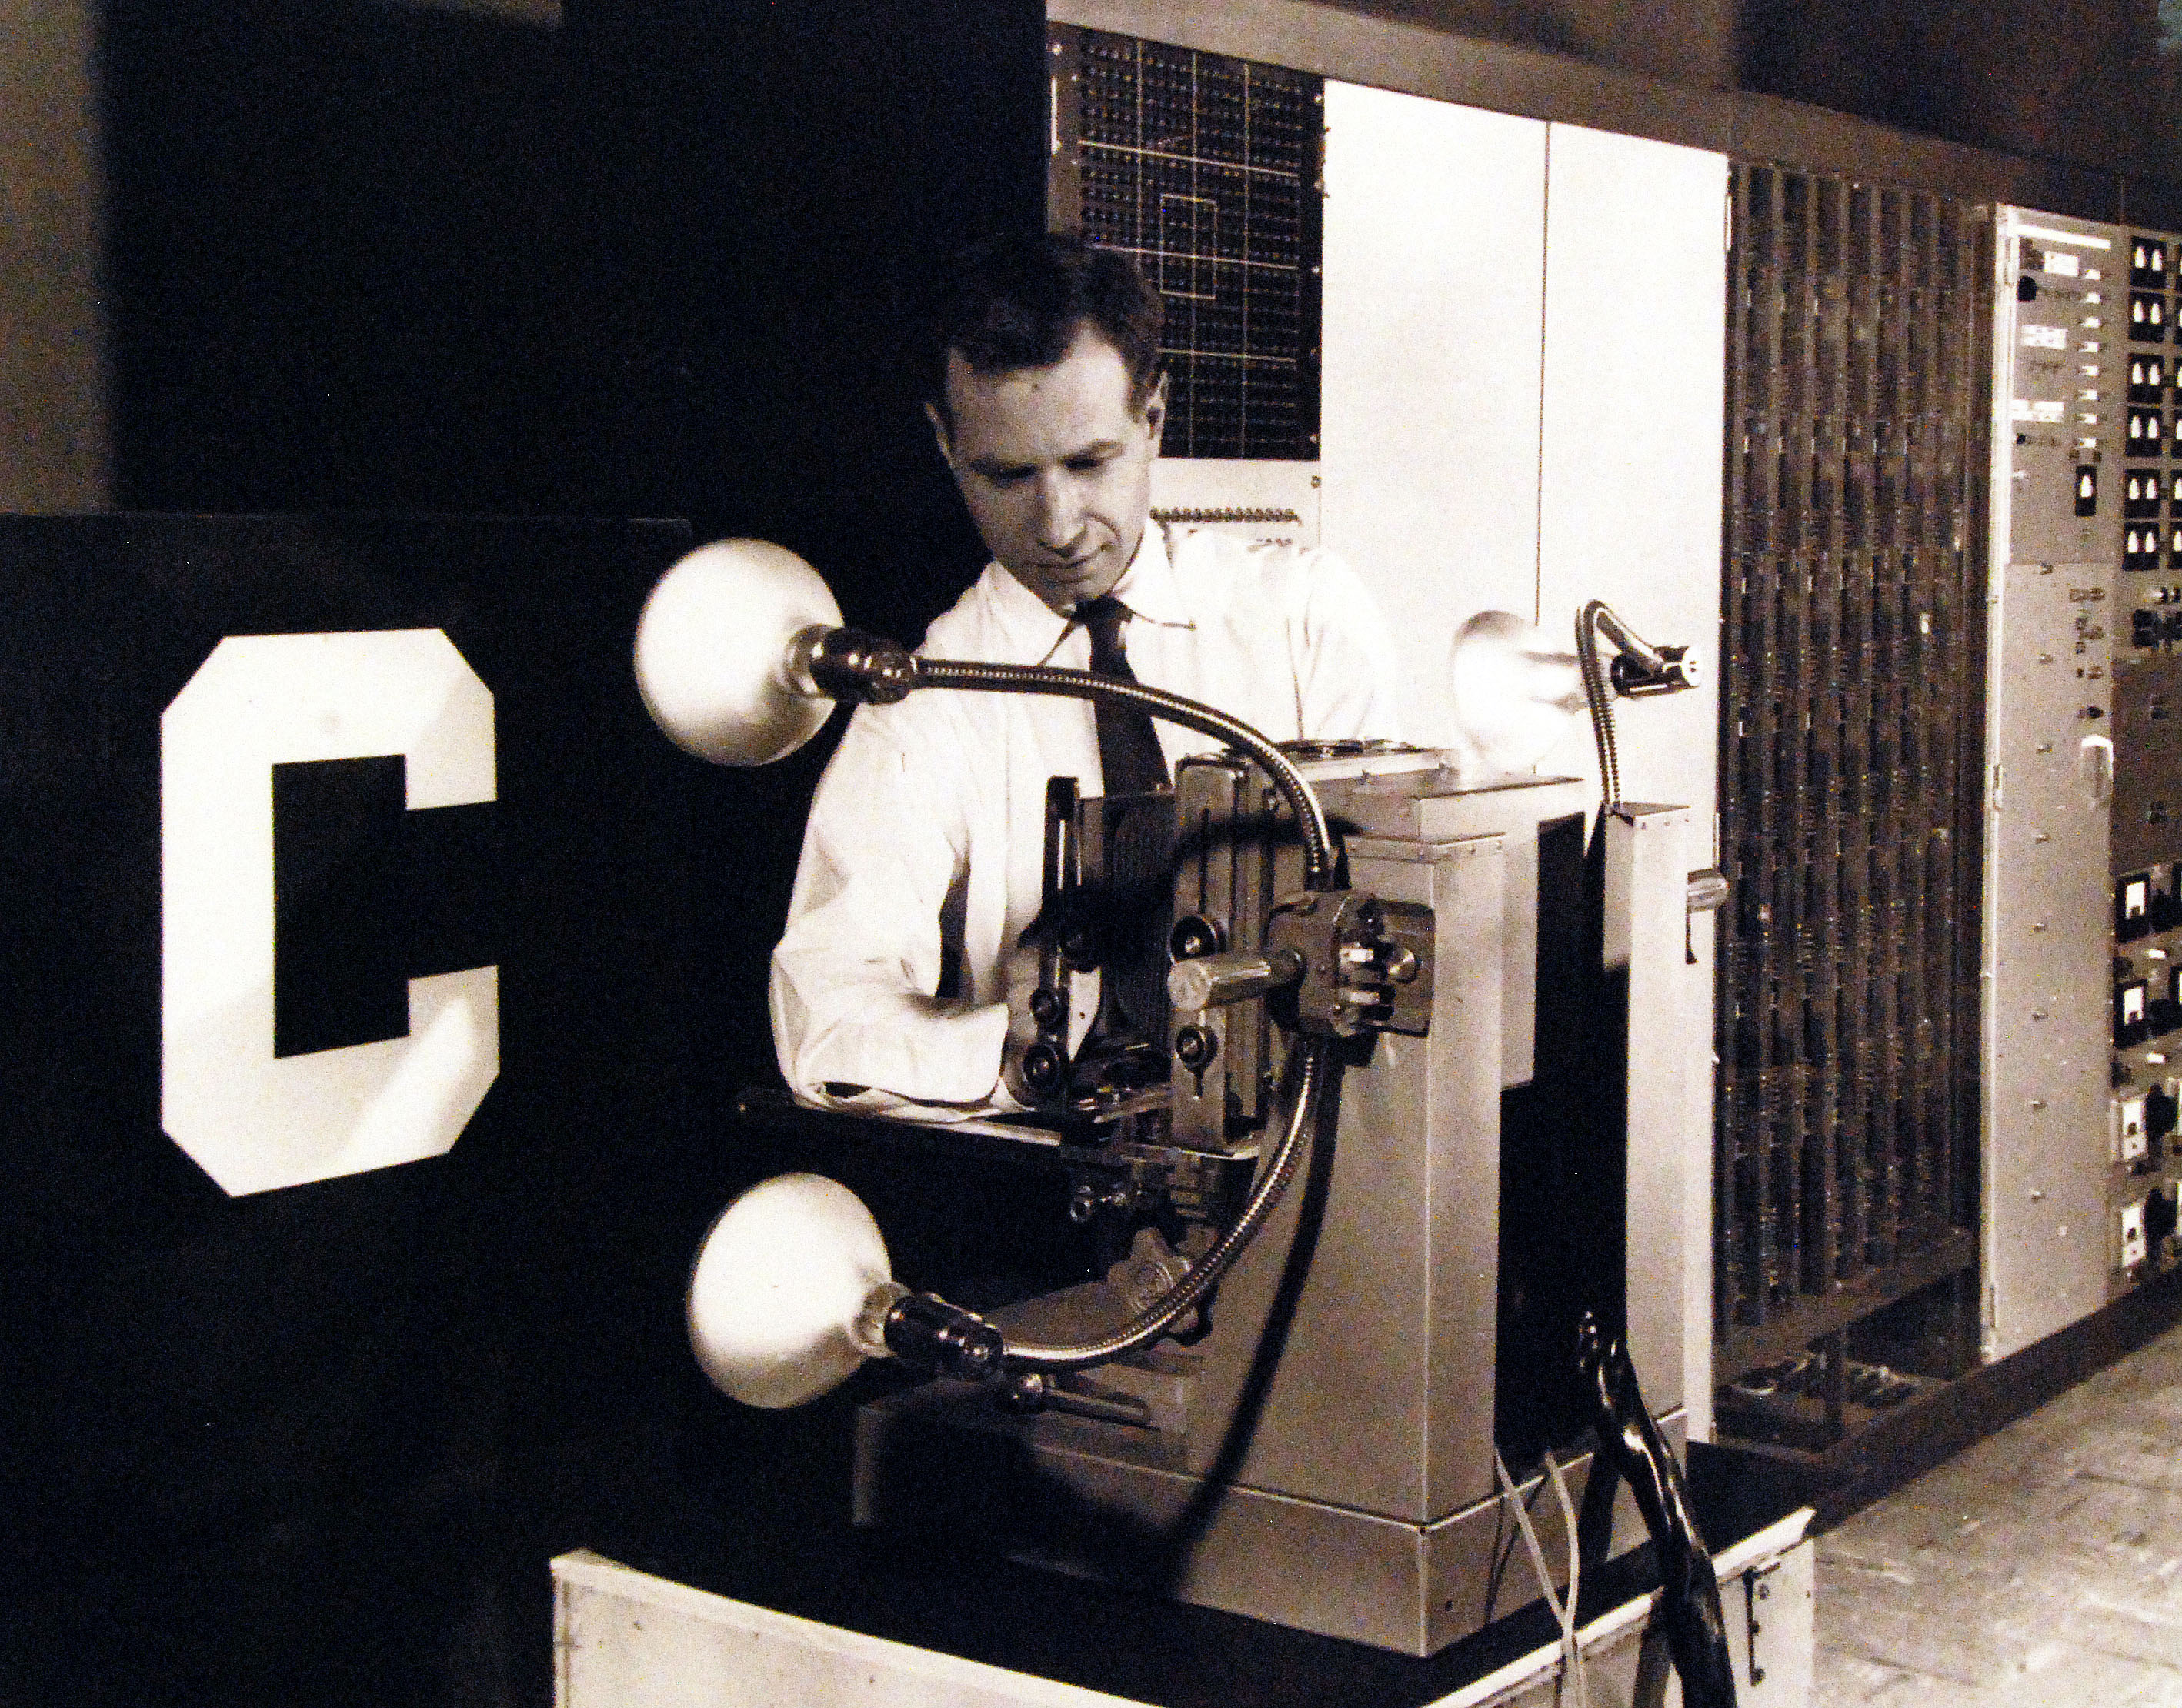
\includegraphics[width=\textwidth]{figuras/rosenblatt_mark1_perceptron.jpg}
        \caption{Fotografía histórica: Frank Rosenblatt y la computadora analógica \textit{Mark I Perceptron} (Laboratorio Aeronáutico de Cornell, 1960; fuente: \textit{US Navy / Wikimedia Commons}).}
        \label{fig:rosenblatt_historia}
    \end{minipage}
\end{figure}

\subsection{Modelo Adaline para Clasificación}
La red Adaline sustituye el aprendizaje discreto por una optimización continua basada en la regla Delta o algoritmo LMS (\textit{Least Mean Squares}) de Widrow-Hoff:
\begin{enumerate}
    \item La función de activación durante la fase de ajuste de pesos es \textbf{lineal}: $Y(x) = W^T X$.
    \item La señal de error se calcula directamente sobre la salida analógica antes de cuantizar:
    \begin{equation}
    e(x) = d(x) - Y(x) = d(x) - W^T X
    \end{equation}
    \item La corrección de pesos minimiza el Error Cuadrático Medio ($J(W) = \frac{1}{2} \sum [d - W^T X]^2$) mediante descenso de gradiente:
    \begin{equation}
    \Delta W_i = \alpha \cdot [d(x) - Y(x)] \cdot X_i, \quad W_i^* = W_i + \Delta W_i
    \end{equation}
    \item Para emitir una clasificación binaria final ('1' o '0'), se aplica una función de umbral sobre la salida lineal:
    \begin{equation}
    \hat{y}_{class} = \begin{cases} 
    1 & \text{si } Y(x) \ge \theta \\ 
    0 & \text{si } Y(x) < \theta 
    \end{cases}
    \end{equation}
    Para etiquetas deseadas $d \in \{0, 1\}$, el umbral teórico de máxima verosimilitud en regresión lineal es $\theta = 0.5$.
\end{enumerate}

\begin{figure}[H]
    \centering
    \begin{minipage}[b]{0.48\textwidth}
        \centering
        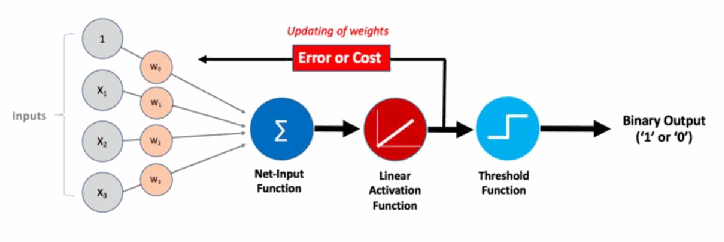
\includegraphics[width=\textwidth]{figuras/modelo_adaline.png}
        \caption{Modelo esquemático de Adaline para clasificación.}
        \label{fig:modelo_adaline}
    \end{minipage}
    \hfill
    \begin{minipage}[b]{0.48\textwidth}
        \centering
        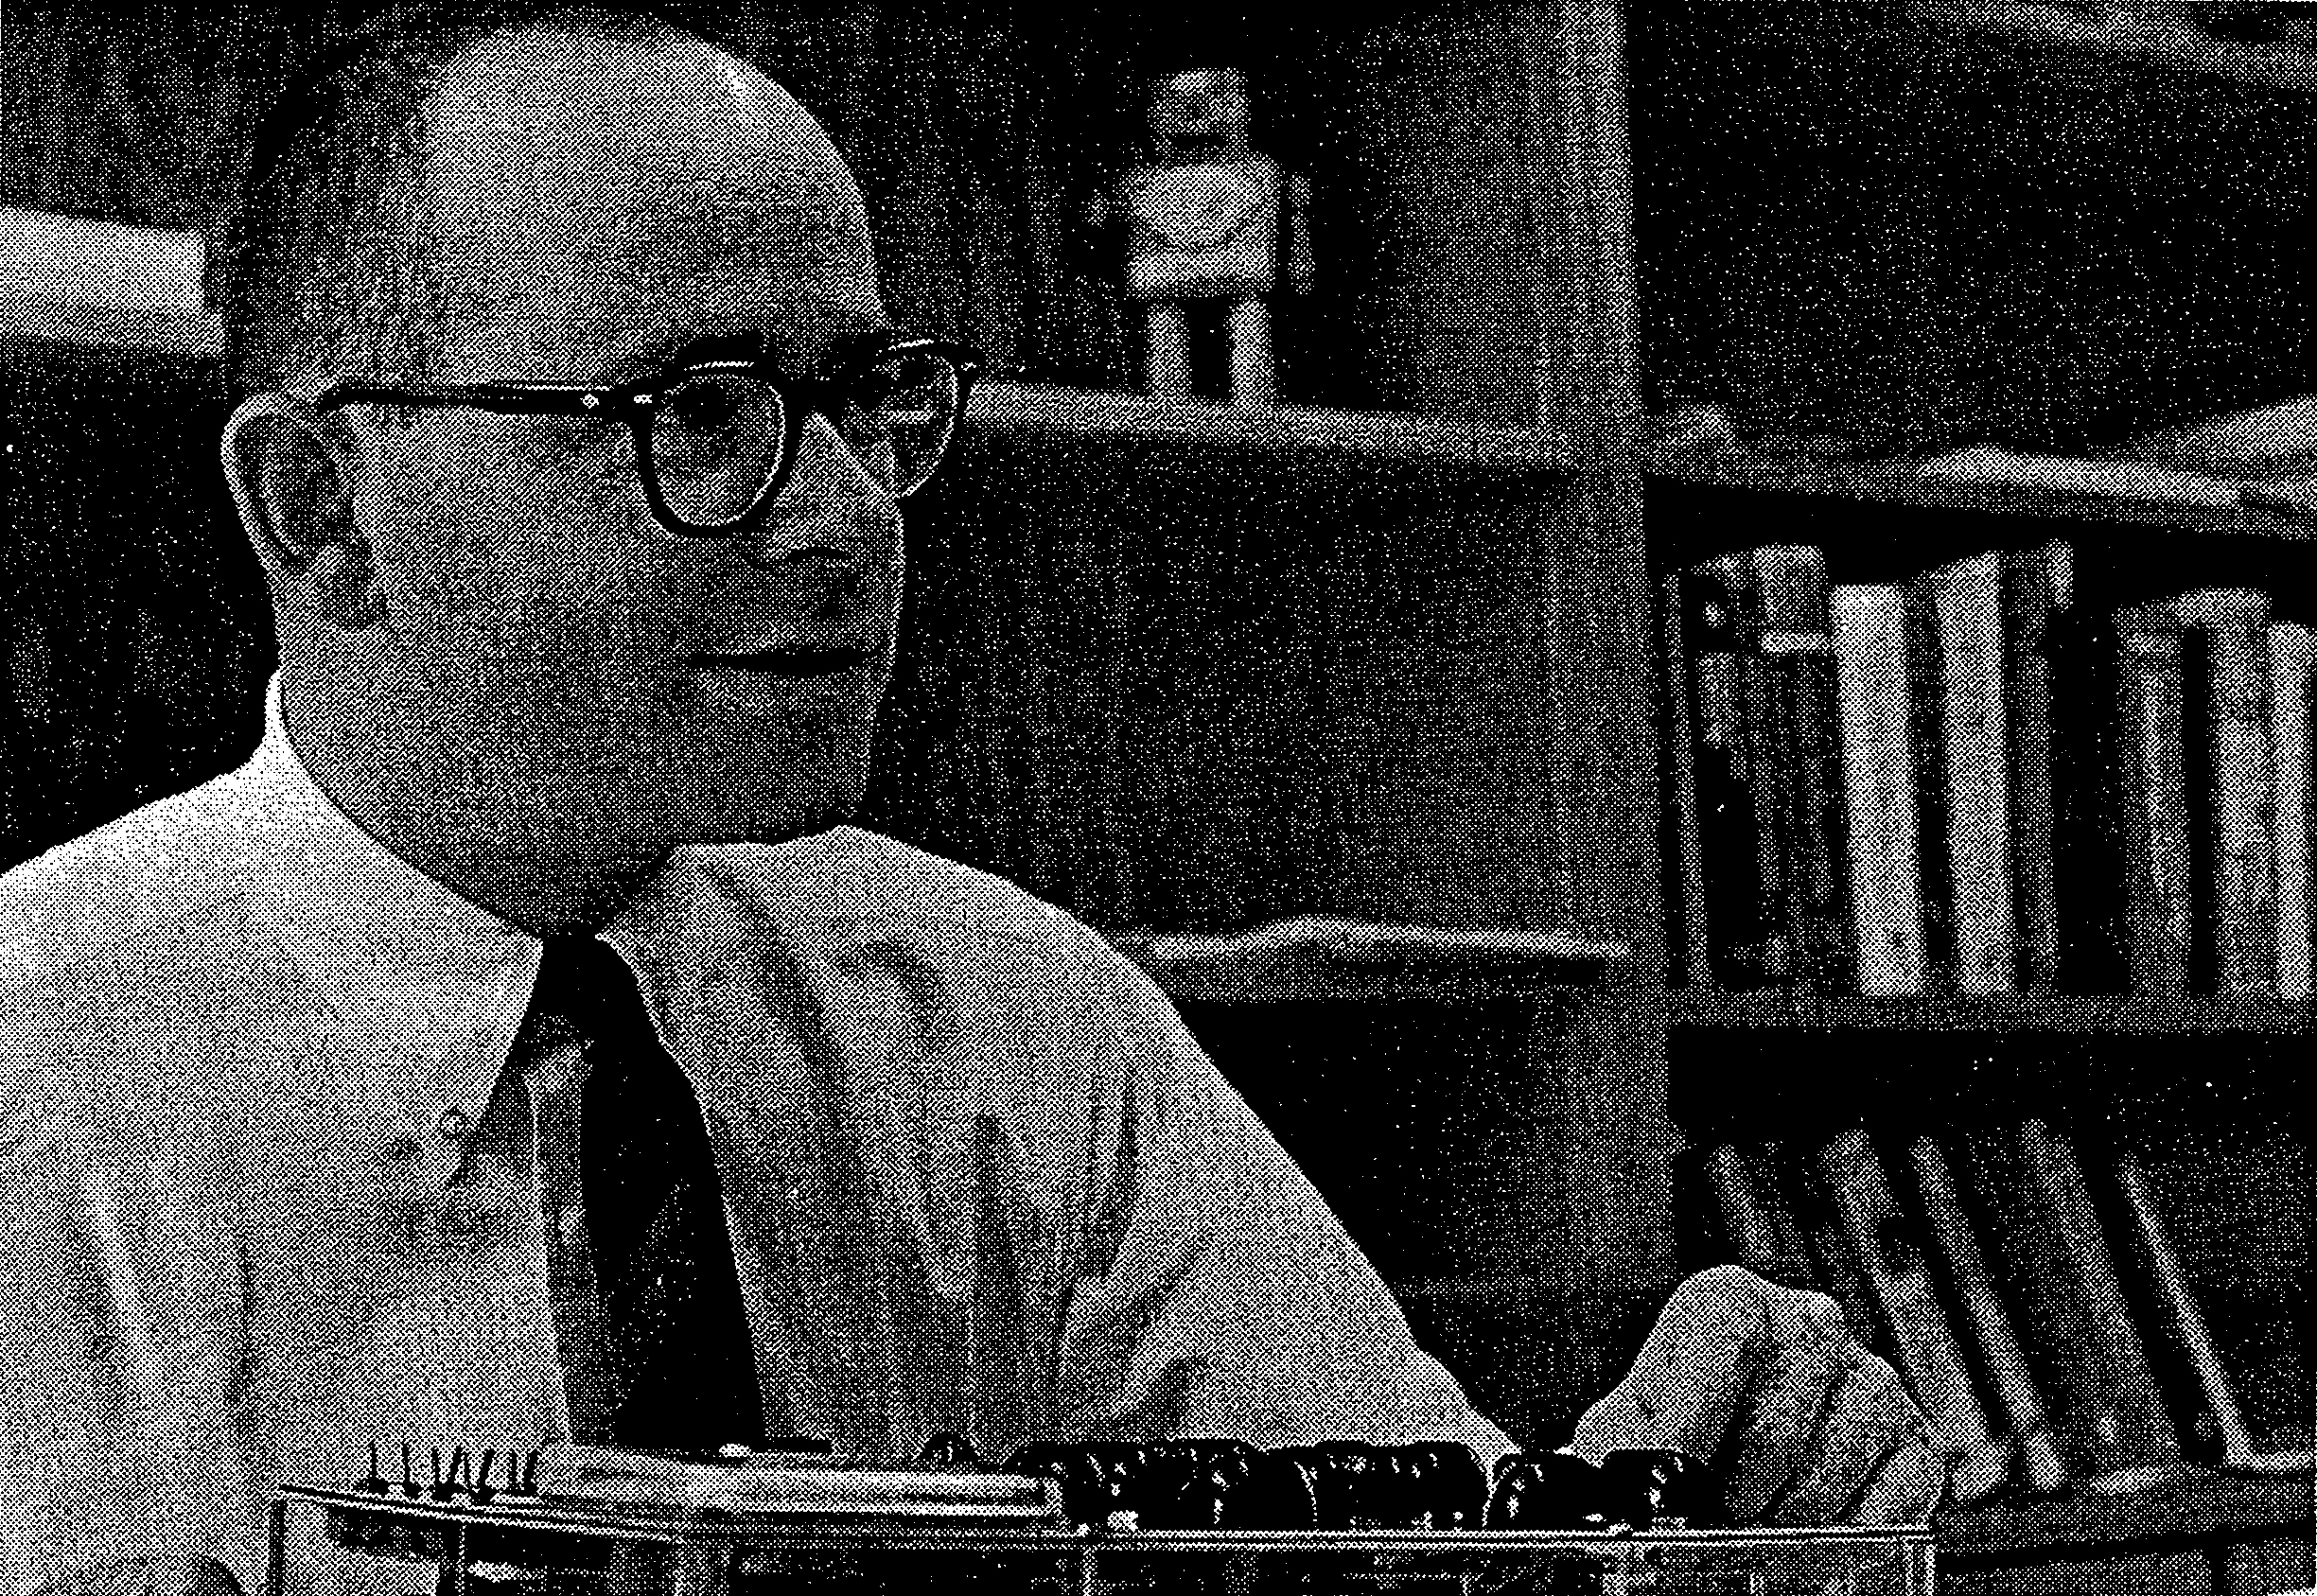
\includegraphics[width=\textwidth]{figuras/bernard_widrow_adaline.jpg}
        \caption{Fotografía histórica: El profesor Bernard Widrow demostrando el hardware original de la red ADALINE basada en memistores (Universidad de Stanford, 1960; fuente: \textit{Stanford University / Wikimedia Commons}).}
        \label{fig:widrow_historia}
    \end{minipage}
\end{figure}

\subsection{Diferencia Estructural Esencial: Bifurcación del Error}
La Figura \ref{fig:tikz_bifurcacion} resume el contraste fundamental entre ambos modelos. Mientras que Adaline extrae el gradiente analítico a partir de la distancia continua $e_{lin} = d(x) - z$, el Perceptrón toma la señal de error $e_{disc} = d(x) - Y_{disc}$ una vez la señal ya ha sido binarizada por el escalón.

\begin{figure}[H]
\centering
\begin{tikzpicture}[scale=0.92, every node/.style={transform shape}]
    % Entradas
    \node[neuron_node] (x0) at (0, 2.2) {$x_0=1$};
    \node[neuron_node] (x1) at (0, 0.9) {$x_1$};
    \node (dots) at (0, -0.2) {$\vdots$};
    \node[neuron_node] (xn) at (0, -1.3) {$x_n$};
    
    % Sumador
    \node[sum_node] (sum) at (4.2, 0.45) {$\sum$};
    
    % Conexiones con pesos
    \draw[arrow] (x0) -- node[above, font=\footnotesize] {$w_0$} (sum);
    \draw[arrow] (x1) -- node[above, font=\footnotesize] {$w_1$} (sum);
    \draw[arrow] (xn) -- node[below, font=\footnotesize] {$w_n$} (sum);
    
    % Punto de bifurcacion
    \coordinate (bifurc) at (6.0, 0.45);
    \draw[thick] (sum) -- (bifurc);
    
    % Rama Adaline (arriba)
    \node[process_green] (adaline_cost) at (6.0, 2.7) {\textbf{Adaline (LMS Widrow-Hoff)}\\Error continuo: $e = d(x) - z$\\$\Delta W_i = \alpha \cdot [d - z] \cdot X_i$};
    \draw[arrow_green] (bifurc) -- (adaline_cost);
    \draw[arrow_green, dashed] (adaline_cost) -| node[above, near start, font=\scriptsize\bfseries, color=green!50!black] {Actualización de Pesos} (2.3, 2.7) -- (2.3, 1.2);
    
    % Escalón Unitario
    \node[func_node] (step) at (8.5, 0.45) {Escalón $\int$};
    \draw[arrow] (bifurc) -- node[above, font=\footnotesize] {$z$} (step);
    
    % Rama Perceptrón (abajo)
    \coordinate (post_step) at (10.5, 0.45);
    \node[process] (percep_cost) at (8.5, -1.9) {\textbf{Perceptrón Simple (Rosenblatt)}\\Error discreto: $e = d(x) - Y$\\$\Delta W_i = \alpha \cdot [d - Y] \cdot X_i$};
    \draw[arrow_blue] (post_step) |- (percep_cost);
    \draw[arrow_blue, dashed] (percep_cost) -| node[below, near start, font=\scriptsize\bfseries, color=blue!60!black] {Actualización de Pesos} (2.3, -1.9) -- (2.3, -0.2);
    
    % Salida final
    \node[font=\bfseries, align=center] (out) at (12.2, 0.45) {Salida Binaria\\$\hat{y} \in \{0, 1\}$};
    \draw[arrow] (step) -- (post_step) -- (out);
\end{tikzpicture}
\caption{Infografía estructural de la bifurcación de la señal de error: Adaline vs Perceptrón Simple.}
\label{fig:tikz_bifurcacion}
\end{figure}

% -------------------------------------------------------------
\section{Metodología de Implementación y Pipeline de Datos}
Toda la lógica computacional fue codificada en Python nativo utilizando las librerías científicas estándar \texttt{NumPy}, \texttt{Pandas}, \texttt{Matplotlib}, \texttt{Seaborn} y \texttt{scikit-learn} (exclusivamente para métricas de validación y carga inicial de datos). Se estructuraron dos clases modulares:
\begin{itemize}
    \item \texttt{PerceptronSimple(n\_inputs, threshold=0.0, rule=3, alpha=0.1, max\_epochs=100)}: Permite configurar el número de entradas, el umbral $\theta$, la regla de corrección (1, 2 o 3), la tasa de aprendizaje $\alpha$, el número máximo de épocas y los pesos iniciales.
    \item \texttt{Adaline(n\_inputs, threshold=0.5, alpha=0.01, max\_epochs=250, tol=1e-5)}: Parametriza el número de variables de entrada, el umbral de corte $\theta$, el factor $\alpha$, la tolerancia de convergencia del MSE y el número de iteraciones máximas.
\end{itemize}

Para garantizar una réplica estricta del protocolo establecido en el archivo de referencia \texttt{Dataset\_train\_test.mlx}, se implementó el pipeline de muestreo sistemático descrito en la Figura \ref{fig:tikz_pipeline}.

\begin{figure}[H]
\centering
\begin{tikzpicture}[scale=0.9, every node/.style={transform shape}]
    \node[startstop] (data) at (0, 0) {Dataset Original\\(Iris / Banknote)};
    \node[process_orange] (seed) at (3.5, 0) {\textbf{Semilla Fija}\\$\text{rng}(2021) \rightarrow \text{randperm}(N)$};
    \node[decision] (split) at (7.7, 0) {Partición\\Porcentual};
    
    % Salidas de particiones
    \node[process] (train) at (12.0, 1.3) {\textbf{Entrenamiento ($Train$)}\\60\%, 70\%, 80\%, 90\%};
    \node[process] (test) at (12.0, -1.3) {\textbf{Prueba ($Test$)}\\40\%, 30\%, 20\%, 10\%};
    
    % Preprocesamiento y Modelos
    \node[process_green] (scale) at (16.2, 0) {\textbf{Estandarización}\\$z = \frac{x - \mu}{\sigma}$};
    
    \draw[arrow] (data) -- (seed);
    \draw[arrow] (seed) -- (split);
    \draw[arrow] (split) |- (train);
    \draw[arrow] (split) |- (test);
    \draw[arrow] (train) -| (scale);
    \draw[arrow] (test) -| (scale);
\end{tikzpicture}
\caption{Pipeline de particionamiento muestral y preprocesamiento de datos según \texttt{Dataset\_train\_test.mlx}.}
\label{fig:tikz_pipeline}
\end{figure}

\subsection{Auditoría y Revisión Estadística de Variables}
Siguiendo la metodología estadística formal establecida para el curso de Inteligencia Computacional, se implementó una auditoría exploratoria y de contraste de hipótesis rigurosa sobre los conjuntos de datos previa al modelado neuronal. El objetivo de este procedimiento es determinar formalmente la ruta analítica (paramétrica vs. no paramétrica), evaluar la relevancia de los atributos frente a la clase, detectar multicolinealidad crítica e identificar la separabilidad espacial intrínseca.

\subsubsection{Protocolo Estadístico y Árbol de Decisión}
La selección de las pruebas de contraste se ejecutó de acuerdo con la siguiente jerarquía de verificación:
\begin{enumerate}
    \item \textbf{Normalidad Univariada y por Clase:} Se contrastó la hipótesis nula de distribución gaussiana mediante la prueba de Shapiro-Wilk y el test conjunto de D'Agostino-Pearson ($K^2$). El rechazo de la hipótesis ($p < 0.05$) descarta el uso de estadística paramétrica estándar.
    \item \textbf{Homocedasticidad (Homogeneidad de Varianzas):} Ante variables continuas se evaluó la igualdad de varianzas entre clases mediante las pruebas de Levene y Fligner-Killeen.
    \item \textbf{Comparación entre Clases:} 
    \begin{itemize}
        \item Si existe normalidad y varianzas homogéneas: $t$-test de Student.
        \item Si existe normalidad pero varianzas heterogéneas: $t$-test de Welch.
        \item Si no existe normalidad: prueba de suma de rangos de Mann-Whitney $U$.
    \end{itemize}
    \item \textbf{Ranking y Relevancia de Atributos:} Medido a través de Información Mutua no lineal ($I(X; Y)$) y estadísticos $F$ de ANOVA / $H$ de Kruskal-Wallis.
    \item \textbf{Multicolinealidad e Inflación de Varianza:} Se calcularon las matrices de correlación de Pearson y Spearman, el Factor de Inflación de la Varianza ($\text{VIF} = \text{diag}(R^{-1})$) y el índice de condición espectral.
    \item \textbf{Detección de Outliers y Balance:} Diagnóstico univariado mediante la regla del Rango Intercuartílico ($1.5 \times \text{IQR}$), outliers multivariados por Distancia de Mahalanobis ($\chi^2$), y balance de clases por test binomial.
\end{enumerate}

\subsubsection{Auditoría Estadística en Banknote Authentication}
La Tabla \ref{tab:eda_banknote} consolida los resultados de la auditoría sobre las 1372 instancias del conjunto de datos de autenticación de billetes bancarios (\textit{Banknote Authentication}).

\begin{table}[H]
\centering
\caption{Auditoría y contraste estadístico de variables en Banknote Authentication.}
\label{tab:eda_banknote}
\begin{adjustbox}{max width=\textwidth}
\begin{tabular}{lcccccccc}
\toprule
\textbf{Variable} & \textbf{Media $\pm$ Std} & \textbf{Shapiro $p$} & \textbf{Levene $p$} & \textbf{Prueba Aplicada} & \textbf{$p$-valor} & \textbf{Info. Mutua} & \textbf{VIF} & \textbf{Outliers (IQR)} \\
\midrule
Varianza  & $0.434 \pm 2.843$ & $4.69 \times 10^{-12}$ & $0.0143$ & Mann-Whitney $U$ & $\mathbf{2.36 \times 10^{-163}}$ & \textbf{0.3780} & 1.531 & 0 \\
Asimetría & $1.922 \pm 5.869$ & $8.22 \times 10^{-15}$ & $0.4793$ & Mann-Whitney $U$ & $\mathbf{8.04 \times 10^{-57}}$  & \textbf{0.2278} & 3.505 & 0 \\
Curtosis  & $1.398 \pm 4.310$ & $2.76 \times 10^{-25}$ & $4.88 \times 10^{-17}$ & Mann-Whitney $U$ & $0.0226$ & 0.1237 & 2.874 & 59 \\
Entropía  & $-1.192 \pm 2.101$ & $4.47 \times 10^{-27}$ & $0.6204$ & Mann-Whitney $U$ & $0.2253$ & 0.0196 & 1.865 & 33 \\
\bottomrule
\end{tabular}
\end{adjustbox}
\end{table}

\textbf{Hallazgos clave:}
\begin{itemize}
    \item \textbf{No normalidad y ruta no paramétrica:} Todas las variables rechazan de forma contundente la hipótesis de normalidad ($p < 10^{-11}$). Por tanto, la comparación estricta exigió Mann-Whitney $U$.
    \item \textbf{Poder discriminante primario:} La Varianza ($p = 2.36 \times 10^{-163}$, $I=0.378$) y la Asimetría ($p = 8.04 \times 10^{-57}$, $I=0.228$) explican la práctica totalidad de la separabilidad entre billetes auténticos y falsos. La Entropía no presenta diferencia estadísticamente significativa de manera aislada ($p = 0.2253$).
    \item \textbf{Ausencia de multicolinealidad perjudicial:} Todos los valores VIF se sitúan por debajo de $3.51$ y el índice de condición es $3.52$, garantizando que los hiperplanos de descenso en Adaline y Perceptrón no sufrirán deformaciones por correlación cruzada.
    \item \textbf{Balance de clases y outliers:} Existen 762 auténticos (55.5\%) y 610 falsificados (44.5\%), un ratio suficientemente balanceado para entrenamiento sin sobremuestreo. Se detectaron únicamente 8 outliers multivariados por distancia de Mahalanobis.
\end{itemize}

\begin{figure}[H]
    \centering
    \begin{minipage}[b]{0.48\textwidth}
        \centering
        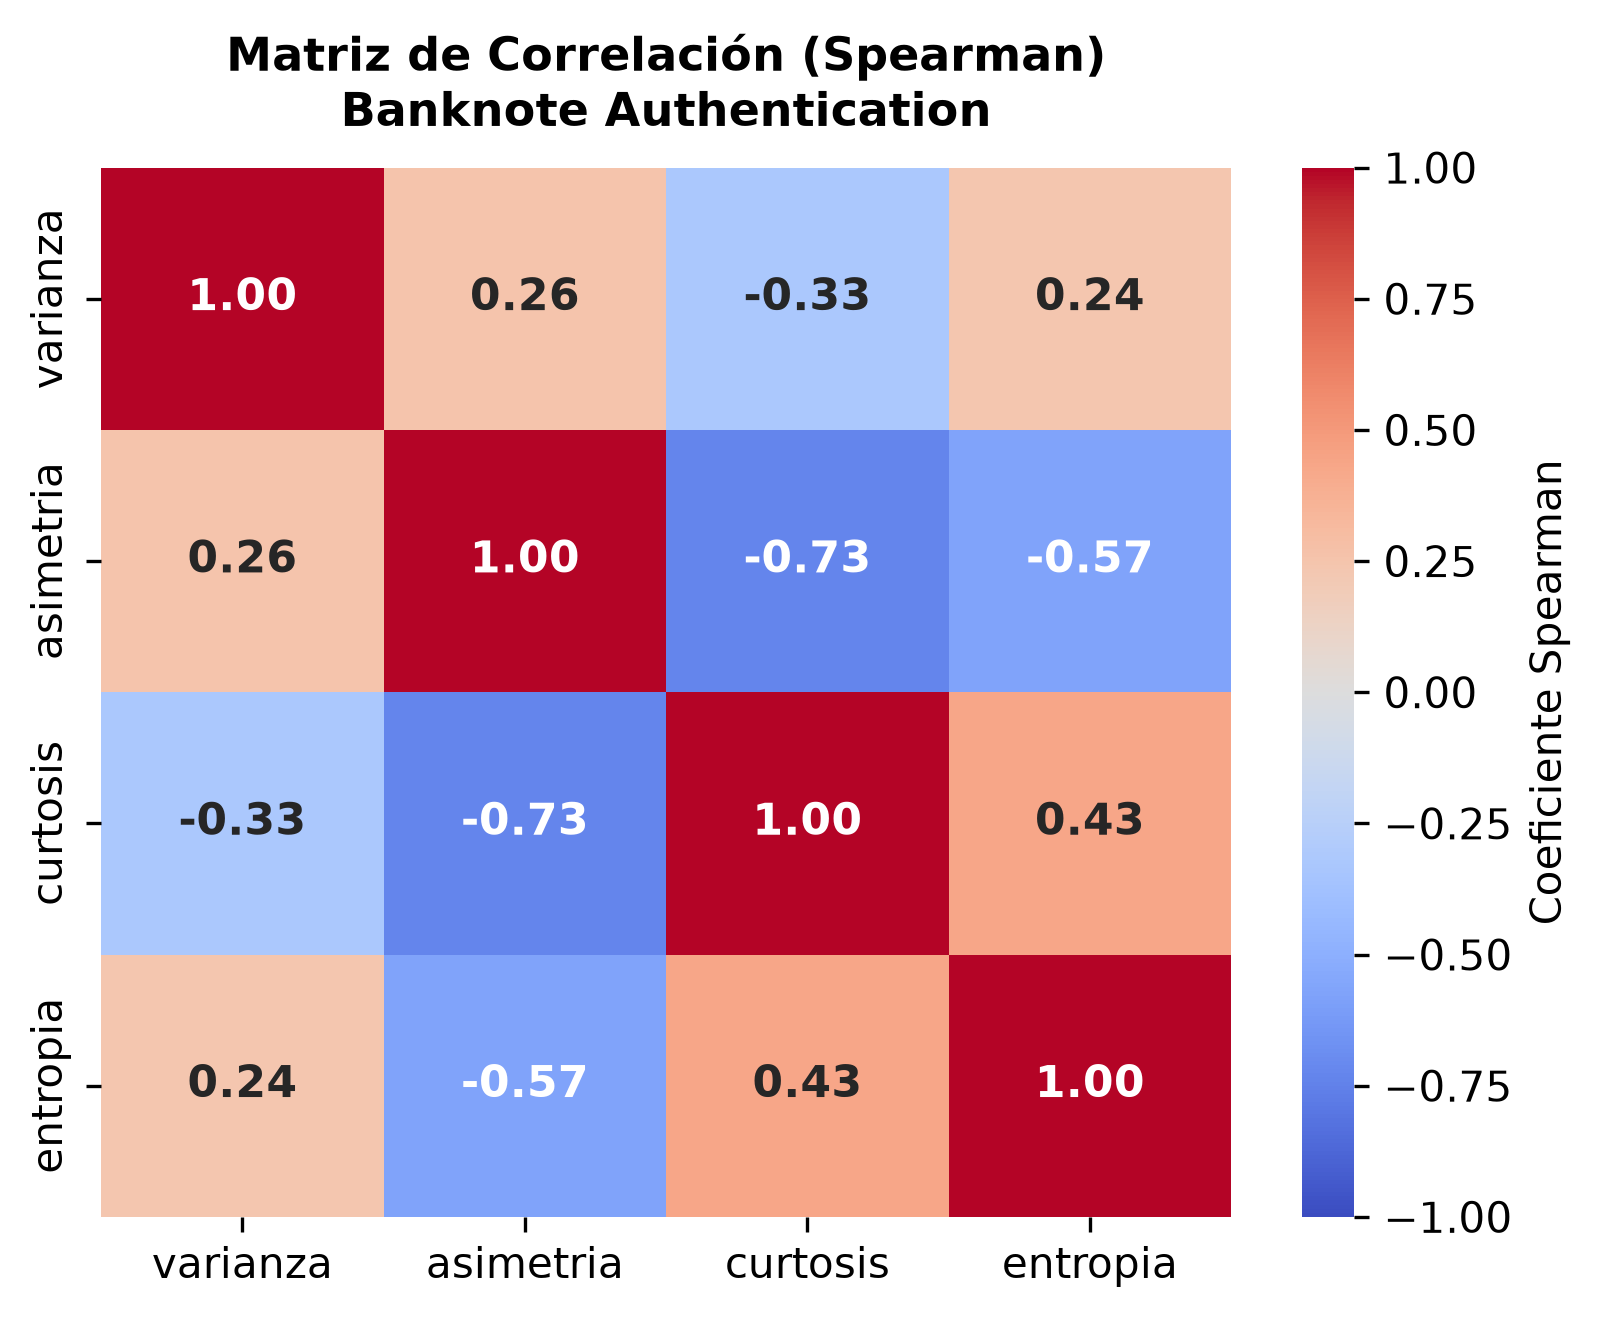
\includegraphics[width=\textwidth]{figuras/eda_banknote_correlacion.png}
        \caption{Matriz de correlación de Pearson y Spearman en Banknote Authentication.}
        \label{fig:eda_bn_corr}
    \end{minipage}
    \hfill
    \begin{minipage}[b]{0.48\textwidth}
        \centering
        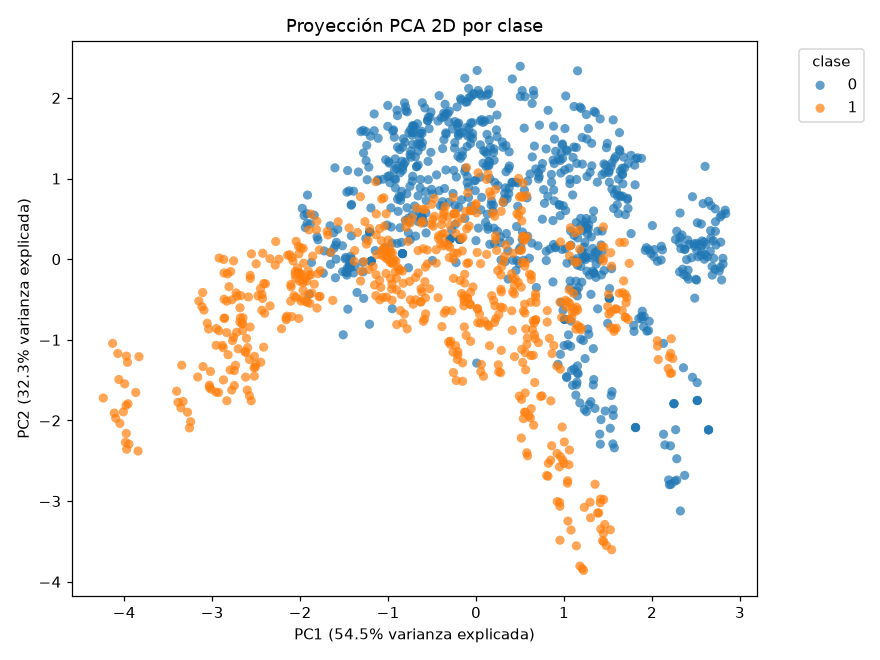
\includegraphics[width=\textwidth]{figuras/eda_banknote_pca.png}
        \caption{Proyección de separabilidad global mediante PCA 2D en Banknote.}
        \label{fig:eda_bn_pca}
    \end{minipage}
\end{figure}

\subsubsection{Auditoría Estadística en Dataset Iris (Setosa vs No-Setosa)}
La Tabla \ref{tab:eda_iris} resume la evaluación sobre el dataset Iris bajo la tarea binaria del taller.

\begin{table}[H]
\centering
\caption{Auditoría y contraste estadístico de variables en Dataset Iris.}
\label{tab:eda_iris}
\begin{adjustbox}{max width=\textwidth}
\begin{tabular}{lcccccccc}
\toprule
\textbf{Variable} & \textbf{Media $\pm$ Std} & \textbf{Shapiro $p$ (0/1)} & \textbf{Levene $p$} & \textbf{Prueba Aplicada} & \textbf{$p$-valor} & \textbf{Info. Mutua} & \textbf{VIF} & \textbf{Outliers (IQR)} \\
\midrule
Long. Sépalo  & $5.843 \pm 0.828$ & $0.146$ / $0.460$ & $7.39 \times 10^{-5}$ & $t$-test de Welch & $\mathbf{7.71 \times 10^{-32}}$ & 0.4063 & 7.073 & 0 \\
Ancho Sépalo  & $3.057 \pm 0.436$ & $0.126$ / $0.272$ & $0.4748$ & $t$-test de Student & $\mathbf{3.06 \times 10^{-16}}$ & 0.2584 & 2.101 & 4 \\
Long. Pétalo  & $3.758 \pm 1.765$ & $0.745$ / $0.055$ & $2.49 \times 10^{-12}$ & $t$-test de Welch & $\mathbf{1.75 \times 10^{-69}}$ & \textbf{0.6399} & \textbf{31.26} & 0 \\
Ancho Pétalo  & $1.199 \pm 0.762$ & $0.001$ / $<10^{-6}$ & $2.81 \times 10^{-15}$ & Mann-Whitney $U$ & $\mathbf{1.33 \times 10^{-23}}$ & \textbf{0.6399} & 16.09 & 0 \\
\bottomrule
\end{tabular}
\end{adjustbox}
\end{table}

\textbf{Hallazgos clave:}
\begin{itemize}
    \item \textbf{Normalidad condicional:} La longitud de sépalo, ancho de sépalo y longitud de pétalo conservan normalidad al evaluarse dentro de cada subgrupo de clase ($p > 0.05$), habilitando la ruta paramétrica ($t$-test de Welch y Student). El ancho de pétalo viola normalidad y se comparó mediante Mann-Whitney $U$.
    \item \textbf{Colinealidad masiva de los pétalos:} Longitud y ancho de pétalo presentan correlación extrema ($r = 0.963$) y VIF muy elevado ($>31$). Ambos comparten la máxima Información Mutua ($0.640$).
    \item \textbf{Separabilidad absoluta:} La proyección de Componentes Principales (Figura \ref{fig:eda_iris_pca}) ilustra que la primera componente principal por sí sola aísla completamente al cluster de \textit{Iris Setosa} respecto a las restantes especies. Esto valida analíticamente por qué tanto el Perceptrón como Adaline convergen en apenas 2 épocas y con 100\% de exactitud.
\end{itemize}

\begin{figure}[H]
    \centering
    \begin{minipage}[b]{0.48\textwidth}
        \centering
        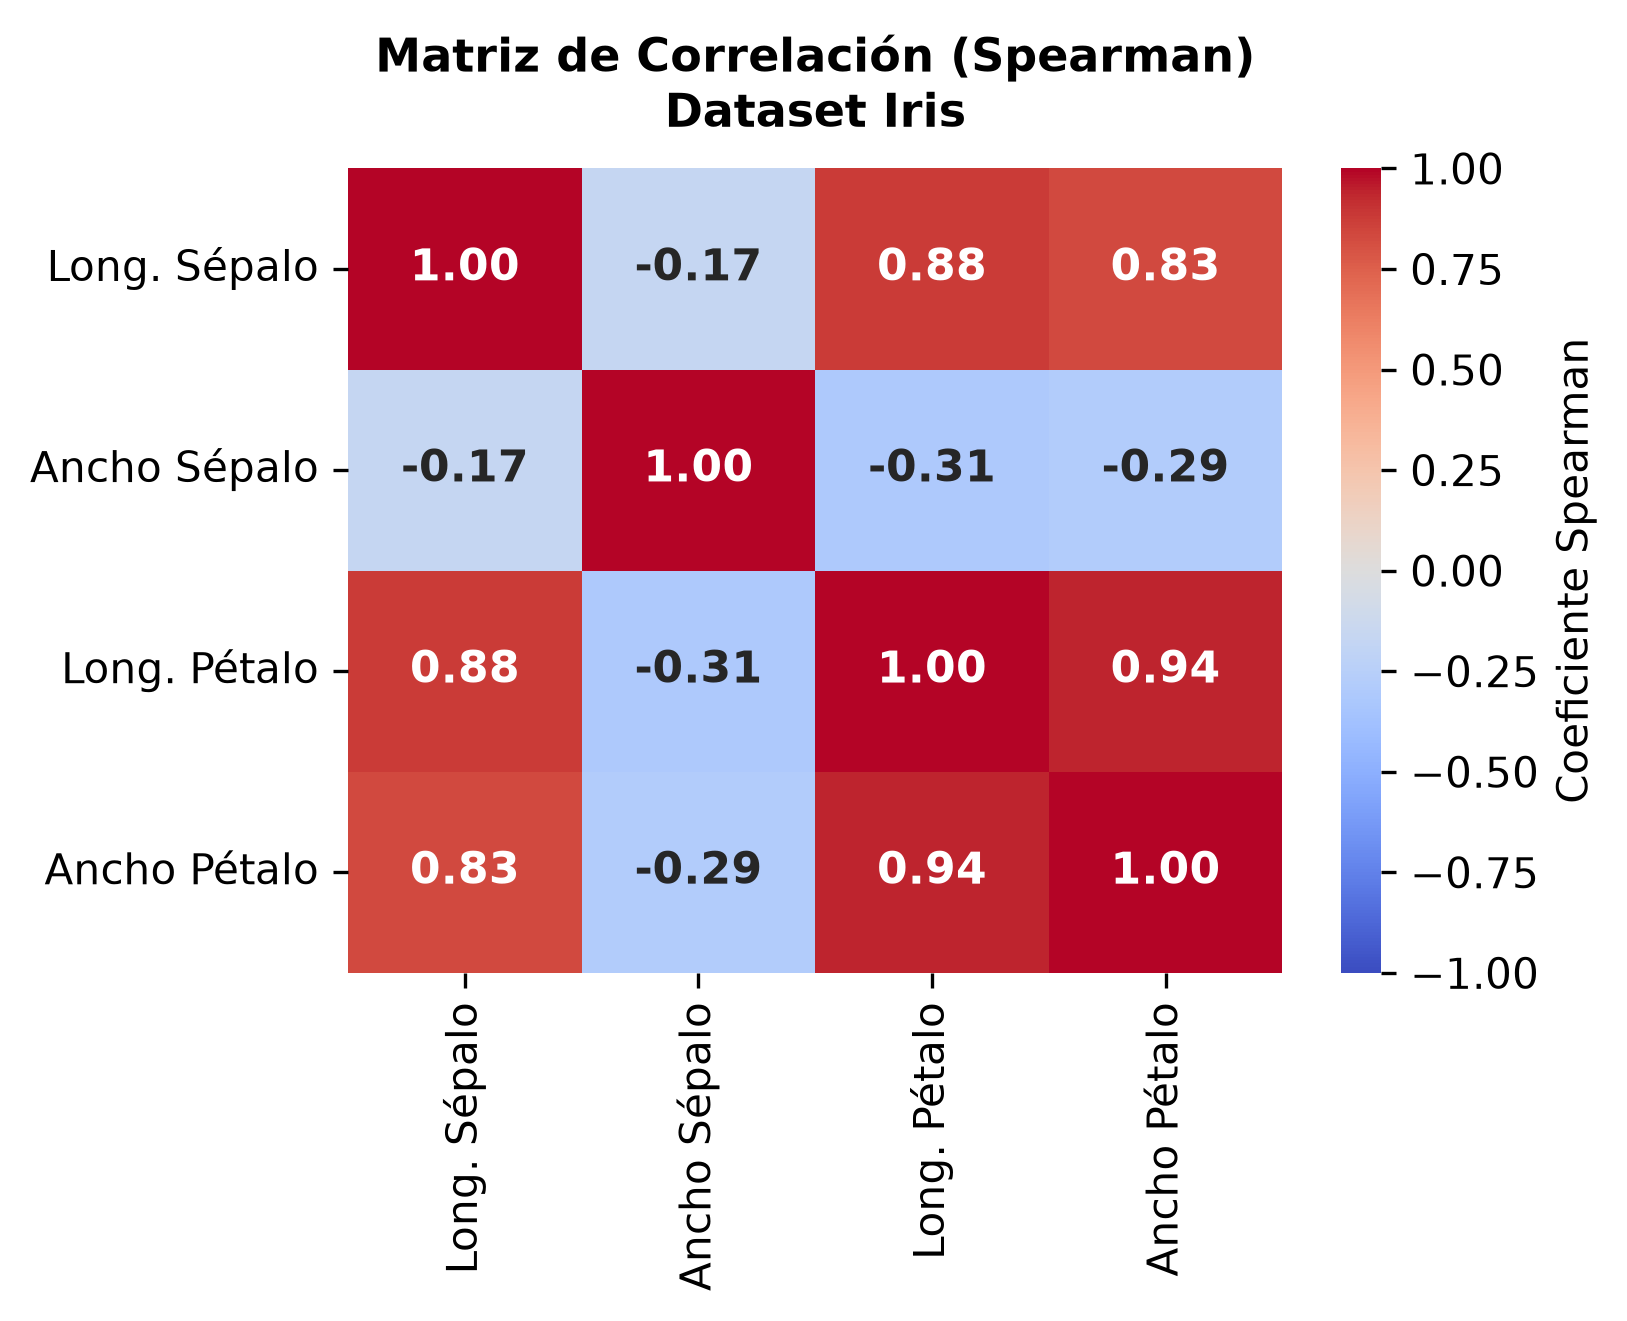
\includegraphics[width=\textwidth]{figuras/eda_iris_correlacion.png}
        \caption{Matriz de correlación de Pearson y Spearman en Dataset Iris.}
        \label{fig:eda_iris_corr}
    \end{minipage}
    \hfill
    \begin{minipage}[b]{0.48\textwidth}
        \centering
        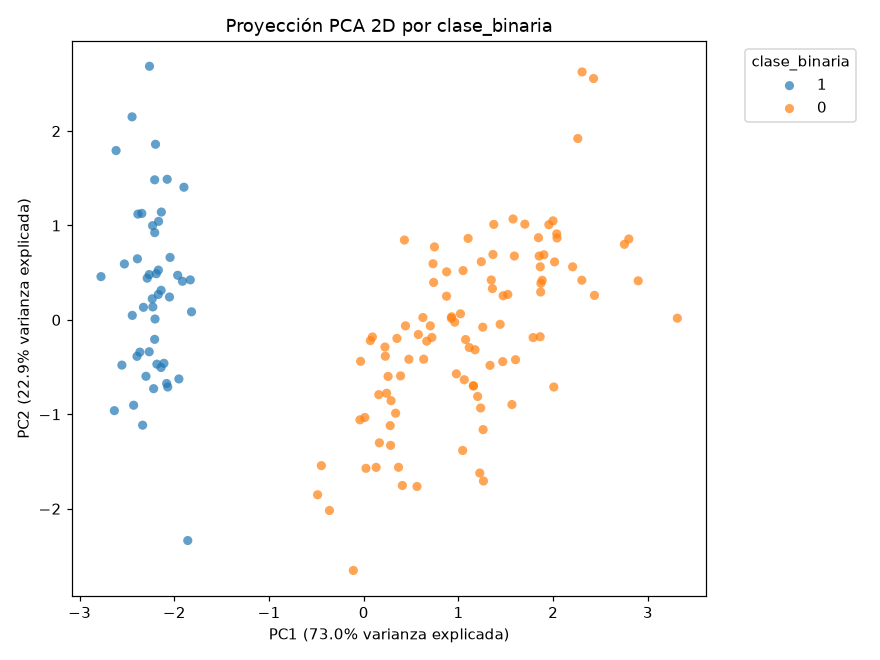
\includegraphics[width=\textwidth]{figuras/eda_iris_pca.png}
        \caption{Proyección PCA 2D confirmando el aislamiento lineal de \textit{Iris Setosa}.}
        \label{fig:eda_iris_pca}
    \end{minipage}
\end{figure}

% -------------------------------------------------------------
\section{Parte I: Experimentación con Perceptrón Simple}

\subsection{Dinámica Algorítmica del Perceptrón}
El algoritmo de entrenamiento del Perceptrón opera de acuerdo al diagrama de flujo de la Figura \ref{fig:tikz_flujo_perceptron}. En cada época, la red recorre secuencialmente los datos y reajusta la orientación del vector de pesos únicamente ante discrepancias entre la salida predicha y la deseada.

\begin{figure}[H]
\centering
\begin{tikzpicture}[scale=0.84, every node/.style={transform shape}]
    \node[startstop] (start) at (0, 0) {Inicio: Parámetros\\$\alpha, \theta, \text{MaxÉpocas}$};
    \node[process] (init) at (0, -1.3) {Inicializar Pesos\\$W = [w_0, w_1, \dots, w_n] \leftarrow 0$};
    \node[process] (sample) at (0, -2.6) {Cargar Patrón\\$(X_k, d_k)$};
    \node[process] (eval) at (0, -3.9) {Calcular Activación\\$z = W^T X_k$, $Y_k = (z \ge \theta)$};
    \node[decision] (check) at (0, -5.5) {¿$Y_k \neq d_k$?};
    \node[process_orange] (update) at (-4.4, -5.5) {Actualizar Pesos\\$W \leftarrow W + \alpha(d_k - Y_k)X_k$\\$\text{errores} \leftarrow \text{errores} + 1$};
    \node[decision] (conv) at (0, -7.6) {¿$\text{errores}=0$\\\textbf{ó} $epoca=\text{Max}$?};
    \node[startstop] (end) at (0, -9.5) {Fin: Modelo Entrenado\\Vector de Pesos $W^*$};
    
    \draw[arrow] (start) -- (init);
    \draw[arrow] (init) -- (sample);
    \draw[arrow] (sample) -- (eval);
    \draw[arrow] (eval) -- (check);
    \draw[arrow] (check) -- node[above, font=\footnotesize\bfseries] {Sí} (update);
    \draw[arrow] (update) |- (sample);
    \draw[arrow] (check) -- node[right, font=\footnotesize\bfseries] {No} (conv);
    \draw[arrow] (conv) -- node[right, font=\footnotesize\bfseries] {Sí} (end);
    \draw[arrow] (conv) -| node[above, near start, font=\footnotesize\bfseries] {No (Siguiente Época)} (4.5, -7.6) |- (sample);
\end{tikzpicture}
\caption{Diagrama de flujo del algoritmo de aprendizaje supervisado del Perceptrón Simple.}
\label{fig:tikz_flujo_perceptron}
\end{figure}

\subsection{Compuertas Lógicas AND y OR (2, 3 y 4 Entradas)}
Se generaron las tablas de verdad completas para $2^2=4$, $2^3=8$ y $2^4=16$ combinaciones booleanas. La Tabla \ref{tab:compuertas_p} consolida el comportamiento de convergencia y exactitud para las tres reglas de actualización bajo $\alpha = 0.1$. Todas las tablas del presente informe han sido ajustadas rigurosamente al ancho de página mediante cajas de redimensionamiento automático.

\begin{table}[H]
\centering
\caption{Resultados del Perceptrón en compuertas lógicas ($\alpha = 0.1$).}
\label{tab:compuertas_p}
\begin{adjustbox}{max width=\textwidth}
\begin{tabular}{lcccccc}
\toprule
\textbf{Compuerta} & \textbf{Entradas} & \textbf{Regla} & \textbf{Épocas} & \textbf{¿Convergió?} & \textbf{Exactitud} & \textbf{Vector de Pesos Final $[w_0, w_1, \dots, w_n]$} \\
\midrule
AND & 2 & Regla 1 & 100 & No & 25.0\% & $[100.0, 100.0, 100.0]$ \\
AND & 2 & Regla 2 & 6 & Sí & 100.0\% & $[-3.0, 2.0, 1.0]$ \\
AND & 2 & Regla 3 & 4 & Sí & 100.0\% & $[-0.2, 0.2, 0.1]$ \\
\midrule
AND & 3 & Regla 1 & 100 & No & 12.5\% & $[100.0, 100.0, 100.0, 100.0]$ \\
AND & 3 & Regla 2 & 7 & Sí & 100.0\% & $[-4.0, 2.0, 1.0, 1.0]$ \\
AND & 3 & Regla 3 & 3 & Sí & 100.0\% & $[-0.2, 0.1, 0.1, 0.1]$ \\
\midrule
AND & 4 & Regla 1 & 100 & No & 6.25\% & $[100.0, 100.0, 100.0, 100.0, 100.0]$ \\
AND & 4 & Regla 2 & 16 & Sí & 100.0\% & $[-8.0, 4.0, 2.0, 1.0, 1.0]$ \\
AND & 4 & Regla 3 & 17 & Sí & 100.0\% & $[-0.8, 0.4, 0.2, 0.1, 0.1]$ \\
\midrule
OR  & 2 & Regla 1 & 100 & No & 75.0\% & $[300.0, 200.0, 200.0]$ \\
OR  & 2 & Regla 2 & 3 & Sí & 100.0\% & $[-1.0, 1.0, 1.0]$ \\
OR  & 2 & Regla 3 & 3 & Sí & 100.0\% & $[-0.1, 0.1, 0.1]$ \\
\midrule
OR  & 3 & Regla 1 & 100 & No & 87.5\% & $[700.0, 400.0, 400.0, 400.0]$ \\
OR  & 3 & Regla 2 & 3 & Sí & 100.0\% & $[-1.0, 1.0, 1.0, 1.0]$ \\
OR  & 3 & Regla 3 & 3 & Sí & 100.0\% & $[-0.1, 0.1, 0.1, 0.1]$ \\
\midrule
OR  & 4 & Regla 1 & 100 & No & 93.75\% & $[1500.0, 800.0, 800.0, 800.0, 800.0]$ \\
OR  & 4 & Regla 2 & 3 & Sí & 100.0\% & $[-1.0, 1.0, 1.0, 1.0, 1.0]$ \\
OR  & 4 & Regla 3 & 3 & Sí & 100.0\% & $[-0.1, 0.1, 0.1, 0.1, 0.1]$ \\
\bottomrule
\end{tabular}
\end{adjustbox}
\end{table}

\begin{figure}[H]
    \centering
    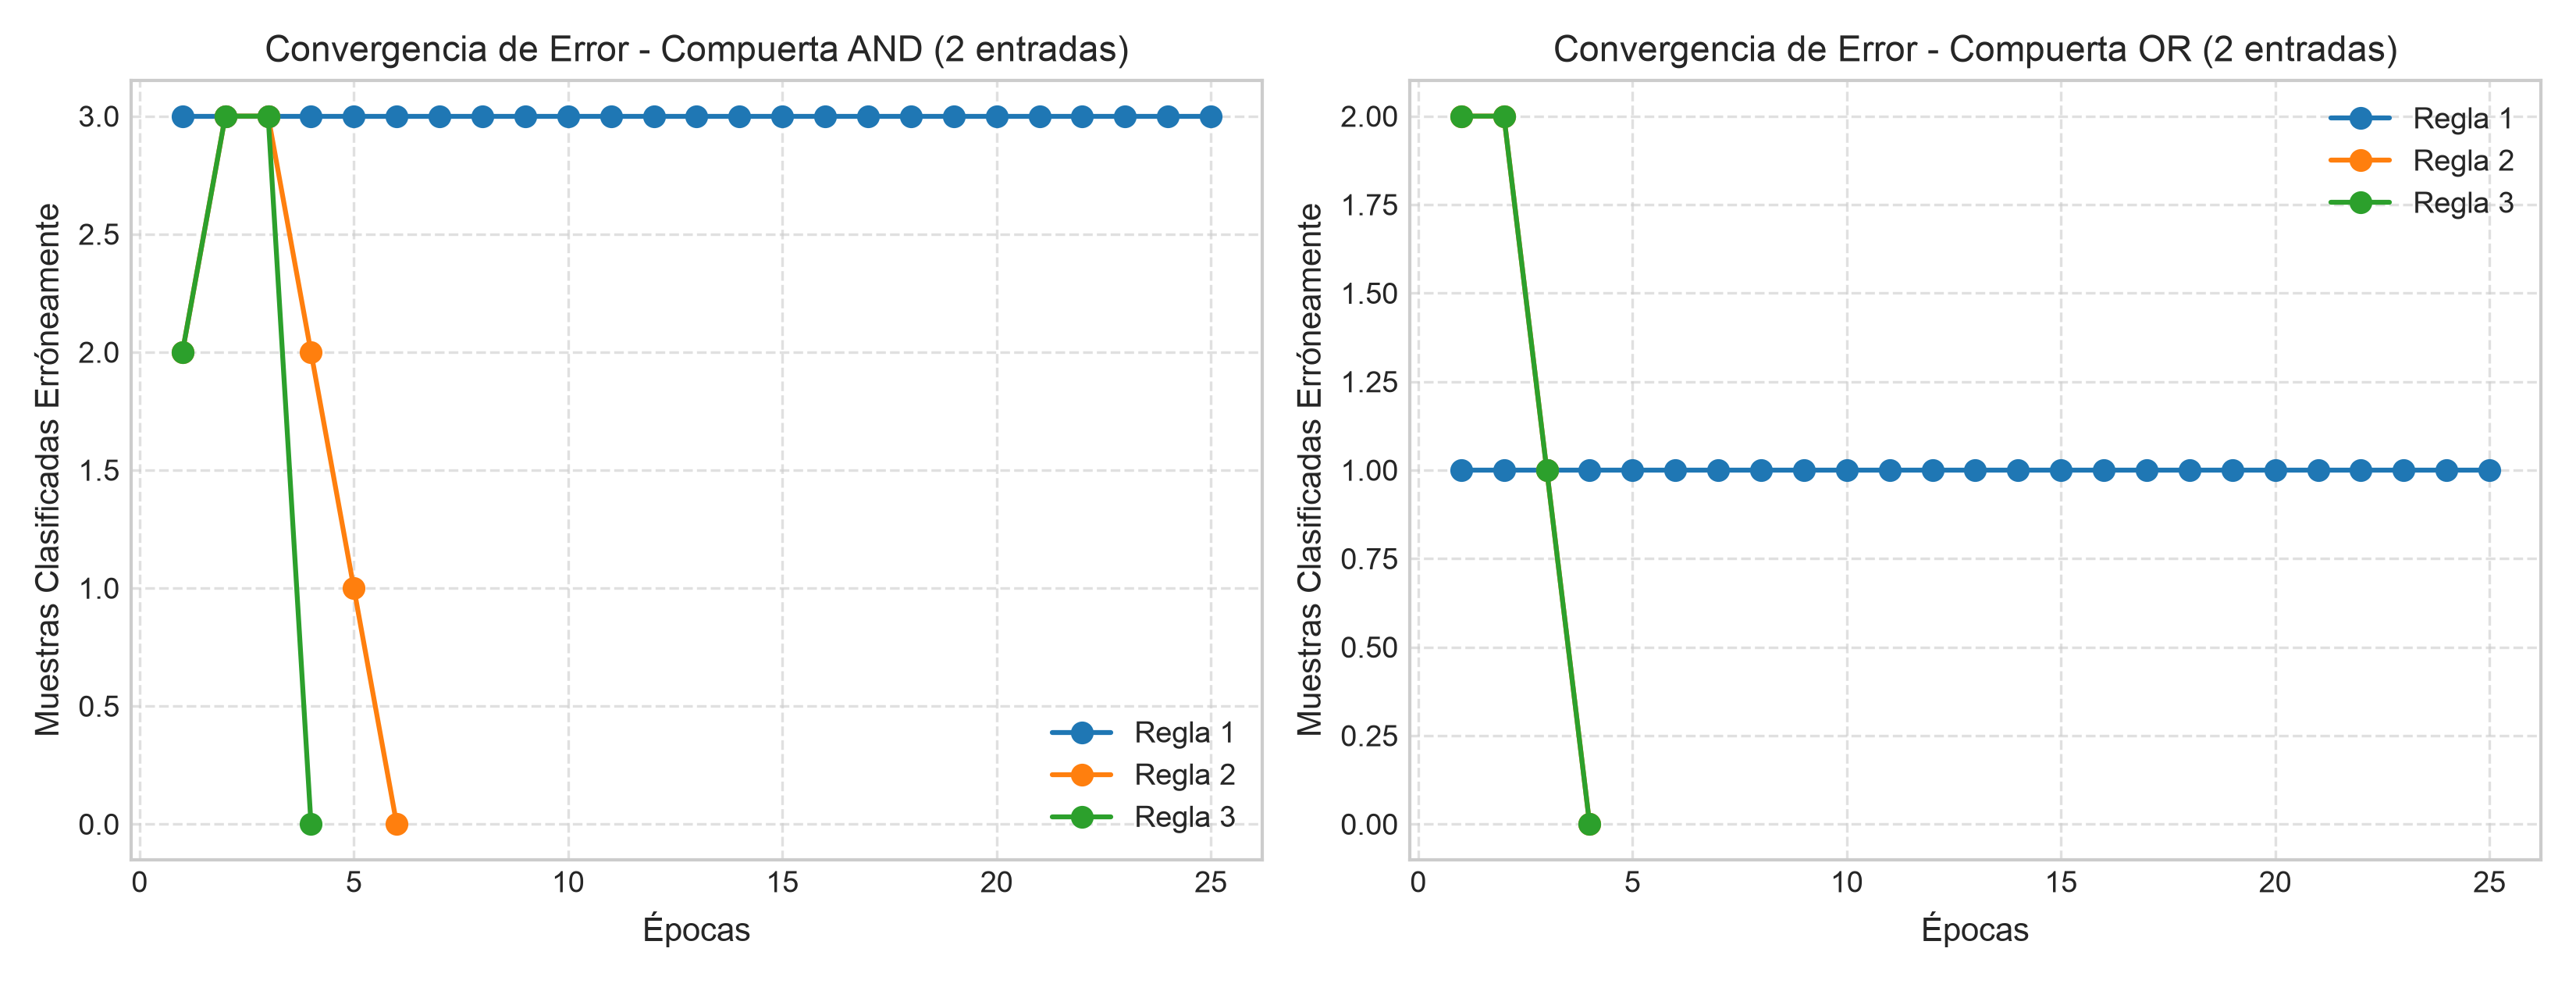
\includegraphics[width=0.88\textwidth]{figuras/reglas_perceptron_comparacion.png}
    \caption{Comparación de convergencia de errores entre Regla 1, Regla 2 y Regla 3 para AND y OR.}
    \label{fig:reglas_p}
\end{figure}

\subsubsection{Justificación Teórica del Comportamiento de las Reglas}
La Figura \ref{fig:reglas_p} ilustra el contraste fundamental entre las tres reglas de aprendizaje:
\begin{itemize}
    \item \textbf{Inviabilidad de la Regla 1 ($\Delta W_i = d(x) \cdot X_i$):} Dado que $d(x) \in \{0, 1\}$ y $X_i \in \{0, 1\}$, la corrección $\Delta W_i$ es siempre estrictamente positiva o cero. Los pesos solo se incrementan ante muestras positivas ($d=1$). Cuando el modelo comete un falso positivo ($Y=1$ cuando $d=0$), la corrección es nula ($\Delta W = 0$). En consecuencia, los pesos aumentan monótonamente hacia el infinito y la frontera de decisión se desplaza alejándose del origen, clasificando todo como $Y=1$. Para compuertas AND de $n$ variables, la exactitud colapsa a $1/2^n$.
    \item \textbf{Eficacia de las Reglas 2 y 3:} Al incorporar el término de error con signo $e = d(x) - Y(x)$, el modelo aplica retroalimentación negativa ($\Delta W < 0$) ante falsos positivos y retroalimentación positiva ($\Delta W > 0$) ante falsos negativos. La Regla 3 modula la amplitud de este salto mediante $\alpha$, permitiendo trayectorias de convergencia más suaves y reduciendo el sobreajuste oscilatorio en las fronteras.
\end{itemize}

\begin{figure}[H]
    \centering
    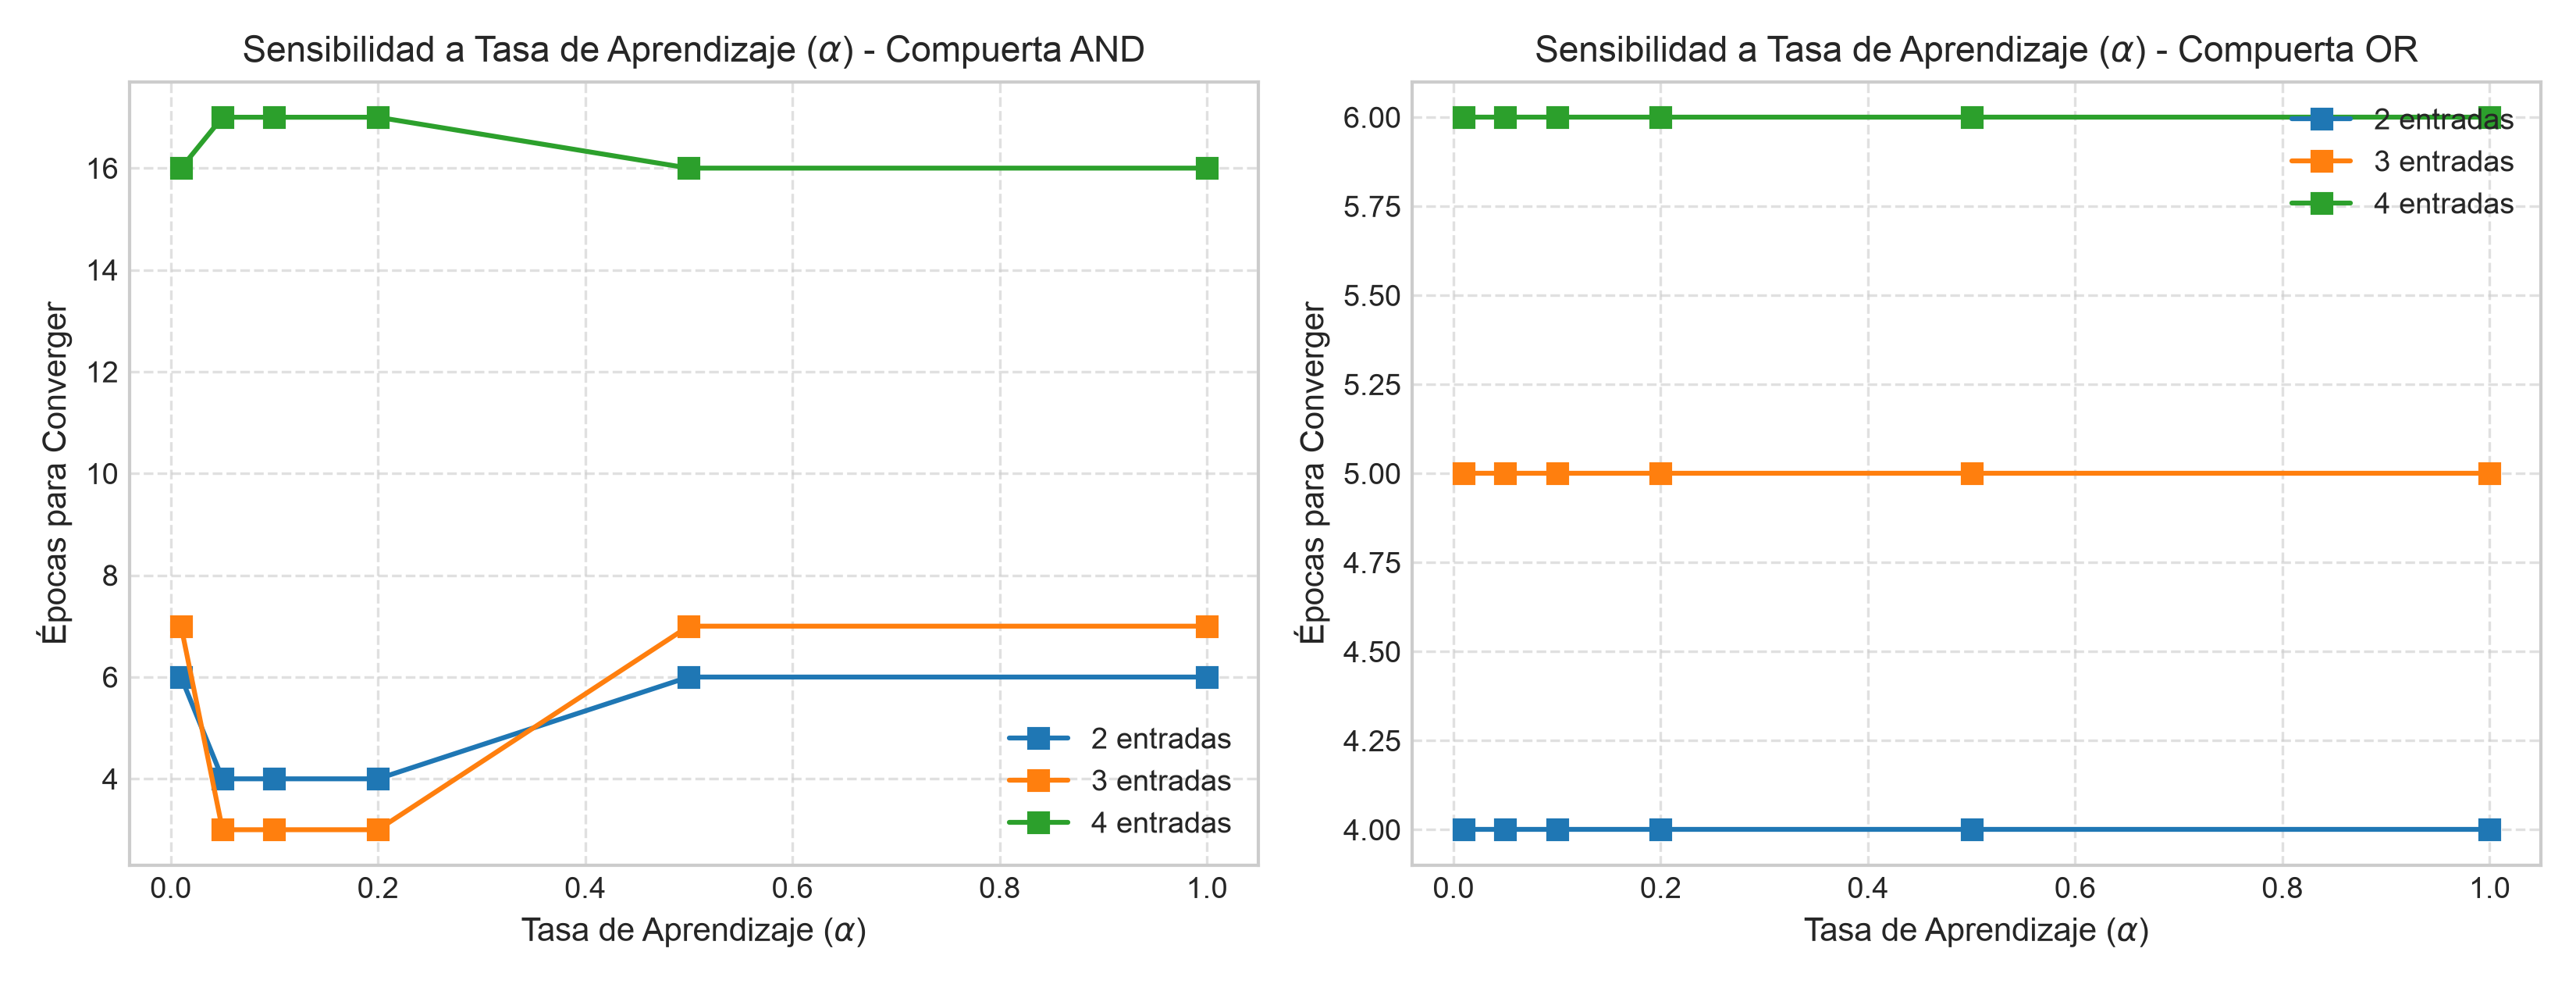
\includegraphics[width=0.85\textwidth]{figuras/compuertas_convergencia_perceptron.png}
    \caption{Sensibilidad del número de épocas de convergencia del Perceptrón en función de $\alpha$.}
    \label{fig:sensibilidad_alpha_p}
\end{figure}

\subsection{Clasificación en Dataset Iris (Punto 4)}
Se evaluó la separabilidad lineal de la especie \textit{Iris Setosa} frente a las restantes dos especies (\textit{Versicolour} y \textit{Virginica}). Se analizaron las particiones 60-40, 70-30, 80-20 y 90-10 con barrido en $\alpha \in [0.001, 0.01, 0.05, 0.1, 0.5, 1.0]$. Los resultados confirman que \textit{Iris Setosa} es perfectamente separable de manera lineal:
\begin{itemize}
    \item En \textbf{todas} las particiones y para todos los valores de $\alpha$, el perceptrón convergió en exactamente \textbf{2 épocas}.
    \item La exactitud en entrenamiento y prueba fue del \textbf{100.0\%} ($Accuracy = 1.0$).
    \item Como se observa en la Figura \ref{fig:iris_p}, el error cae a cero inmediatamente tras el primer pase completo de los patrones, verificando la amplia distancia de margen existente entre los atributos de \textit{Setosa} respecto a las demás especies.
\end{itemize}

\begin{figure}[H]
    \centering
    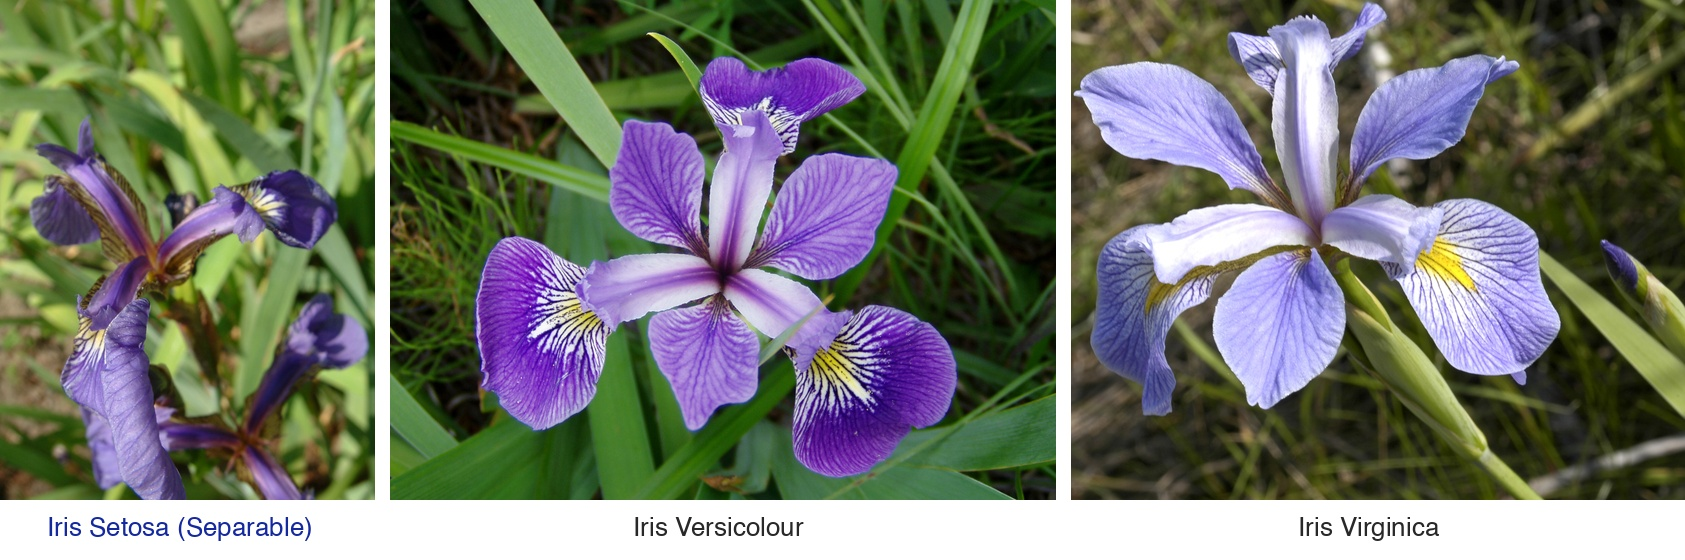
\includegraphics[width=0.88\textwidth]{figuras/iris_especies_comparativa.jpg}
    \caption{Comparación morfológica botánica de las tres especies del dataset Iris: \textit{Iris Setosa} (izquierda), \textit{Iris Versicolour} (centro) e \textit{Iris Virginica} (derecha). La marcada reducción métrica en la longitud y anchura del pétalo de \textit{Setosa} fundamenta físicamente la existencia de un hiperplano de separación lineal perfecto (fuente: \textit{Wikimedia Commons / Botanical Taxonomy}).}
    \label{fig:iris_flores}
\end{figure}

\begin{figure}[H]
    \centering
    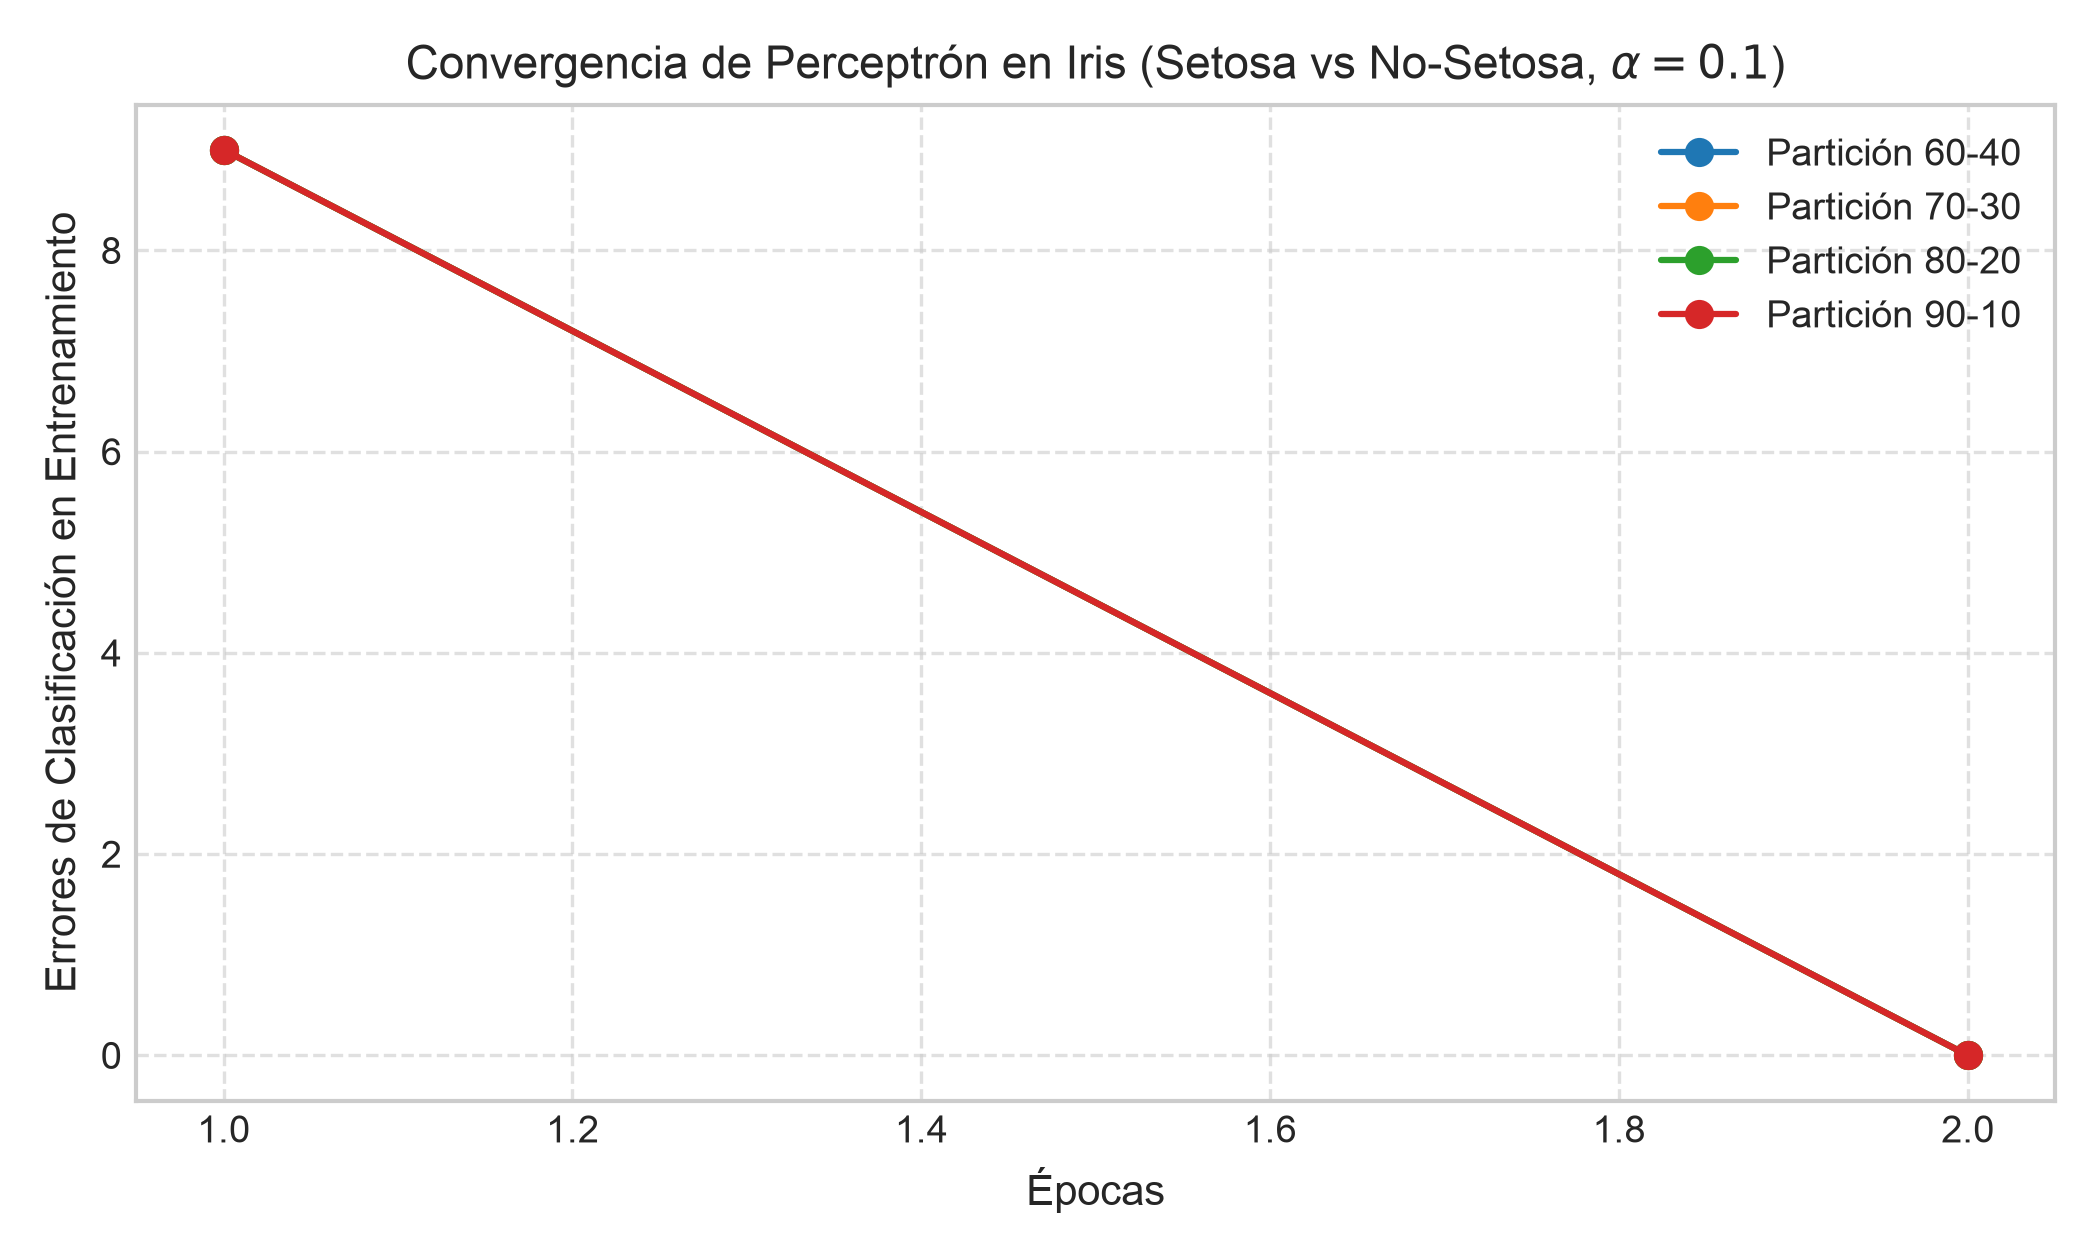
\includegraphics[width=0.60\textwidth]{figuras/iris_convergencia_perceptron.png}
    \caption{Curva de convergencia de errores del Perceptrón en el dataset Iris bajo distintas particiones ($\alpha = 0.1$).}
    \label{fig:iris_p}
\end{figure}

\subsection{Clasificación en Banknote Authentication (Puntos 5 y 6)}
El dataset de autenticación de billetes bancarios (\texttt{data\_banknote\_authentication.txt}) contiene 1372 observaciones continuas de 4 variables físicas. Se estandarizaron las características a media cero y varianza unitaria para optimizar la convergencia geométrica. La Tabla \ref{tab:banknote_p} sintetiza los resultados obtenidos con la Regla 3 ($\alpha = 0.05$).

\begin{table}[H]
\centering
\caption{Métricas de evaluación del Perceptrón en Banknote Authentication ($\alpha = 0.05$).}
\label{tab:banknote_p}
\begin{adjustbox}{max width=\textwidth}
\begin{tabular}{lccccccc}
\toprule
\textbf{Partición} & \textbf{Muestras Train} & \textbf{Muestras Test} & \textbf{Exactitud Train} & \textbf{Exactitud Test} & \textbf{Precisión} & \textbf{Sensibilidad (Recall)} & \textbf{F1-Score} \\
\midrule
60-40 & 823 & 549 & 99.15\% & 99.27\% & 98.39\% & 100.0\% & 0.9919 \\
70-30 & 960 & 412 & 98.44\% & 98.06\% & 98.33\% & 97.25\% & 0.9779 \\
80-20 & 1097 & 275 & 99.00\% & 97.82\% & 95.20\% & 100.0\% & 0.9754 \\
90-10 & 1234 & 138 & 99.03\% & 99.28\% & 100.0\% & 98.28\% & 0.9913 \\
\bottomrule
\end{tabular}
\end{adjustbox}
\end{table}

\begin{figure}[H]
    \centering
    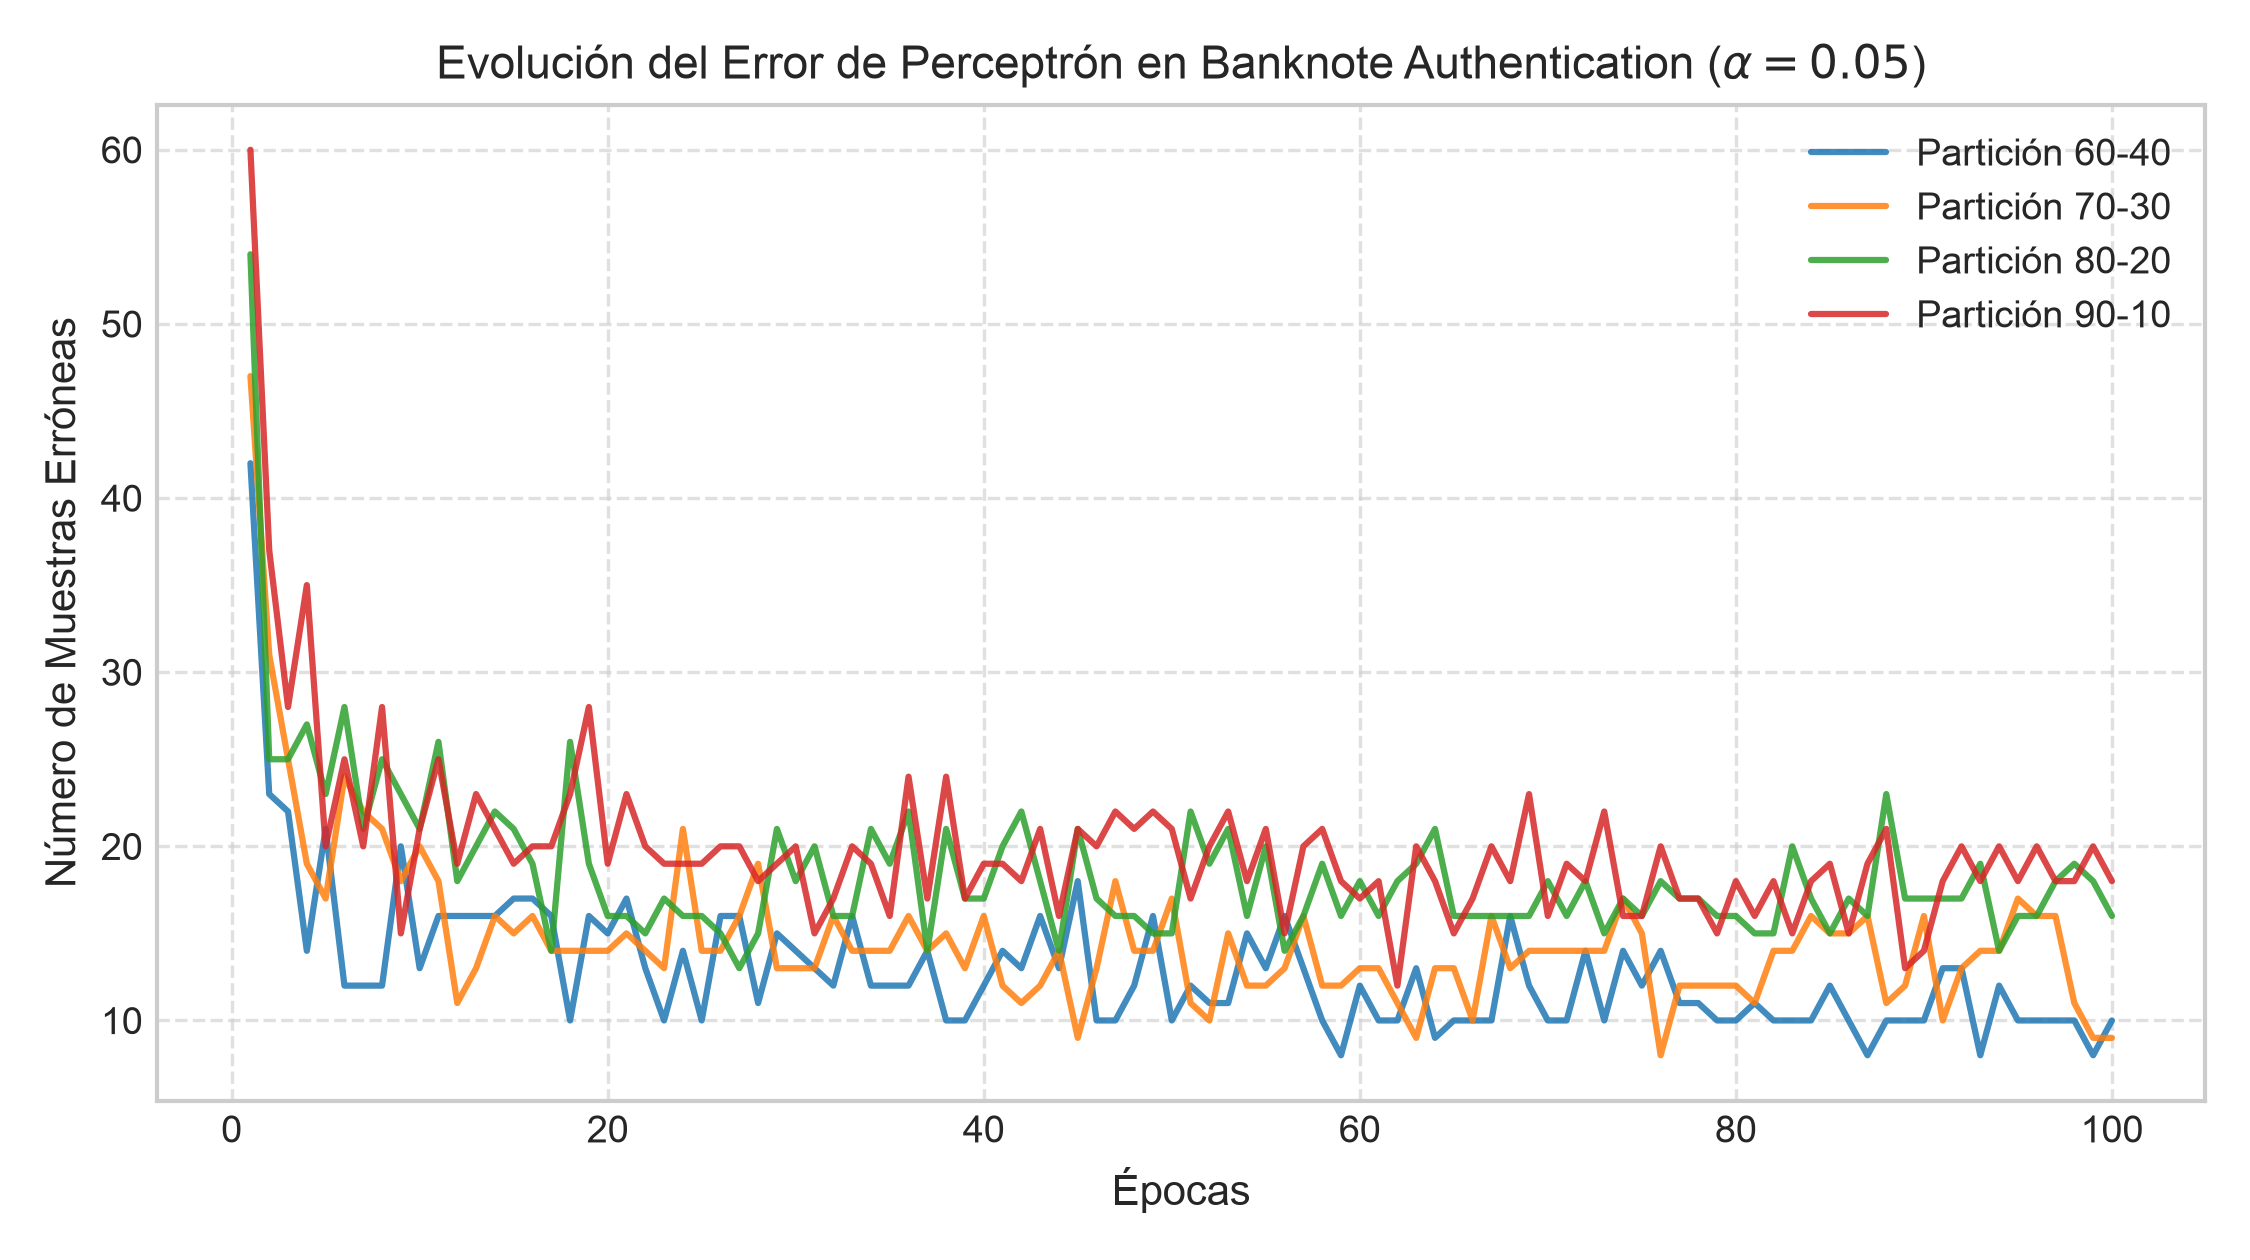
\includegraphics[width=0.68\textwidth]{figuras/banknote_convergencia_perceptron.png}
    \caption{Evolución del número de muestras mal clasificadas en Banknote Authentication ($\alpha = 0.05$).}
    \label{fig:banknote_p}
\end{figure}

% -------------------------------------------------------------
\section{Parte II: Experimentación con Red Adaline}

\subsection{Dinámica Algorítmica de Adaline}
El flujo operativo de la red Adaline se detalla en la Figura \ref{fig:tikz_flujo_adaline}. A diferencia del perceptrón, Adaline no depende de errores discretos de clasificación para activar su aprendizaje; en su lugar, computa de forma ininterrumpida las correcciones proporcionales al residuo cuadrático continuo.

\begin{figure}[H]
\centering
\begin{tikzpicture}[scale=0.80, every node/.style={transform shape}]
    \node[startstop] (start) at (0, 0) {Inicio: Parámetros\\$\alpha, \theta, \text{tol}, \text{MaxÉpocas}$};
    \node[process_green] (norm) at (0, -1.3) {Estandarización de Datos\\$X_{norm} \leftarrow (X - \mu)/\sigma$};
    \node[process] (init) at (0, -2.6) {Inicializar Pesos\\$W \leftarrow 0$};
    \node[process] (sample) at (0, -3.9) {Cargar Patrón\\$(X_k, d_k)$};
    \node[process_green] (linear) at (0, -5.3) {Salida Lineal Continua\\$Y_k = W^T X_k$, Error: $e_k = d_k - Y_k$};
    \node[process_orange] (lms) at (0, -6.8) {Corrección LMS (Delta)\\$W \leftarrow W + \alpha \cdot e_k \cdot X_k$};
    \node[process] (mse) at (0, -8.3) {Calcular MSE de Época\\$MSE = \frac{1}{N}\sum (d_k - W^T X_k)^2$};
    \node[decision] (stop) at (0, -10.2) {¿$|\Delta MSE| < \text{tol}$\\\textbf{ó} $epoca=\text{Max}$?};
    \node[process] (thresh) at (0, -12.1) {Clasificación por Umbral\\$\hat{y} = (W^T X \ge \theta)$};
    \node[startstop] (end) at (0, -13.6) {Fin: Modelo Entrenado};
    
    \draw[arrow] (start) -- (norm);
    \draw[arrow] (norm) -- (init);
    \draw[arrow] (init) -- (sample);
    \draw[arrow] (sample) -- (linear);
    \draw[arrow] (linear) -- (lms);
    \draw[arrow] (lms) -- (mse);
    \draw[arrow] (mse) -- (stop);
    \draw[arrow] (stop) -- node[right, font=\footnotesize\bfseries] {Sí} (thresh);
    \draw[arrow] (thresh) -- (end);
    \draw[arrow] (stop) -| node[above, near start, font=\footnotesize\bfseries] {No (Siguiente Época)} (4.6, -10.2) |- (sample);
\end{tikzpicture}
\caption{Diagrama de flujo del algoritmo de aprendizaje Adaline con optimización LMS.}
\label{fig:tikz_flujo_adaline}
\end{figure}

\subsection{Compuertas Lógicas AND y OR (Puntos 7, 8 y 9)}
En la Tabla \ref{tab:compuertas_a} se presentan las métricas para $\alpha = 0.1$ con umbral de binarización $\theta = 0.5$.

\begin{table}[H]
\centering
\caption{Resultados de Adaline en compuertas lógicas ($\alpha = 0.1$, umbral $\theta = 0.5$).}
\label{tab:compuertas_a}
\begin{adjustbox}{max width=\textwidth}
\begin{tabular}{lcccccc}
\toprule
\textbf{Compuerta} & \textbf{Entradas} & \textbf{Épocas} & \textbf{MSE Final} & \textbf{¿MSE Convergió?} & \textbf{Exactitud} & \textbf{Pesos Finales $[w_0, w_1, \dots, w_n]$} \\
\midrule
AND & 2 & 39 & 0.06326 & Sí & 100.0\% & $[-0.2404, 0.5282, 0.4997]$ \\
AND & 3 & 19 & 0.06776 & Sí & 100.0\% & $[-0.2712, 0.3420, 0.2918, 0.2620]$ \\
AND & 4 & 14 & 0.06082 & Sí & 100.0\% & $[-0.2945, 0.3084, 0.2236, 0.1803, 0.1567]$ \\
\midrule
OR  & 2 & 56 & 0.06379 & Sí & 100.0\% & $[0.2830, 0.4407, 0.4683]$ \\
OR  & 3 & 7  & 0.06513 & Sí & 87.5\%  & $[0.5189, 0.1891, 0.2175, 0.2318]$ \\
OR  & 4 & 20 & 0.04633 & Sí & 93.75\% & $[0.7244, 0.0735, 0.0843, 0.0907, 0.0939]$ \\
\bottomrule
\end{tabular}
\end{adjustbox}
\end{table}

\begin{figure}[H]
    \centering
    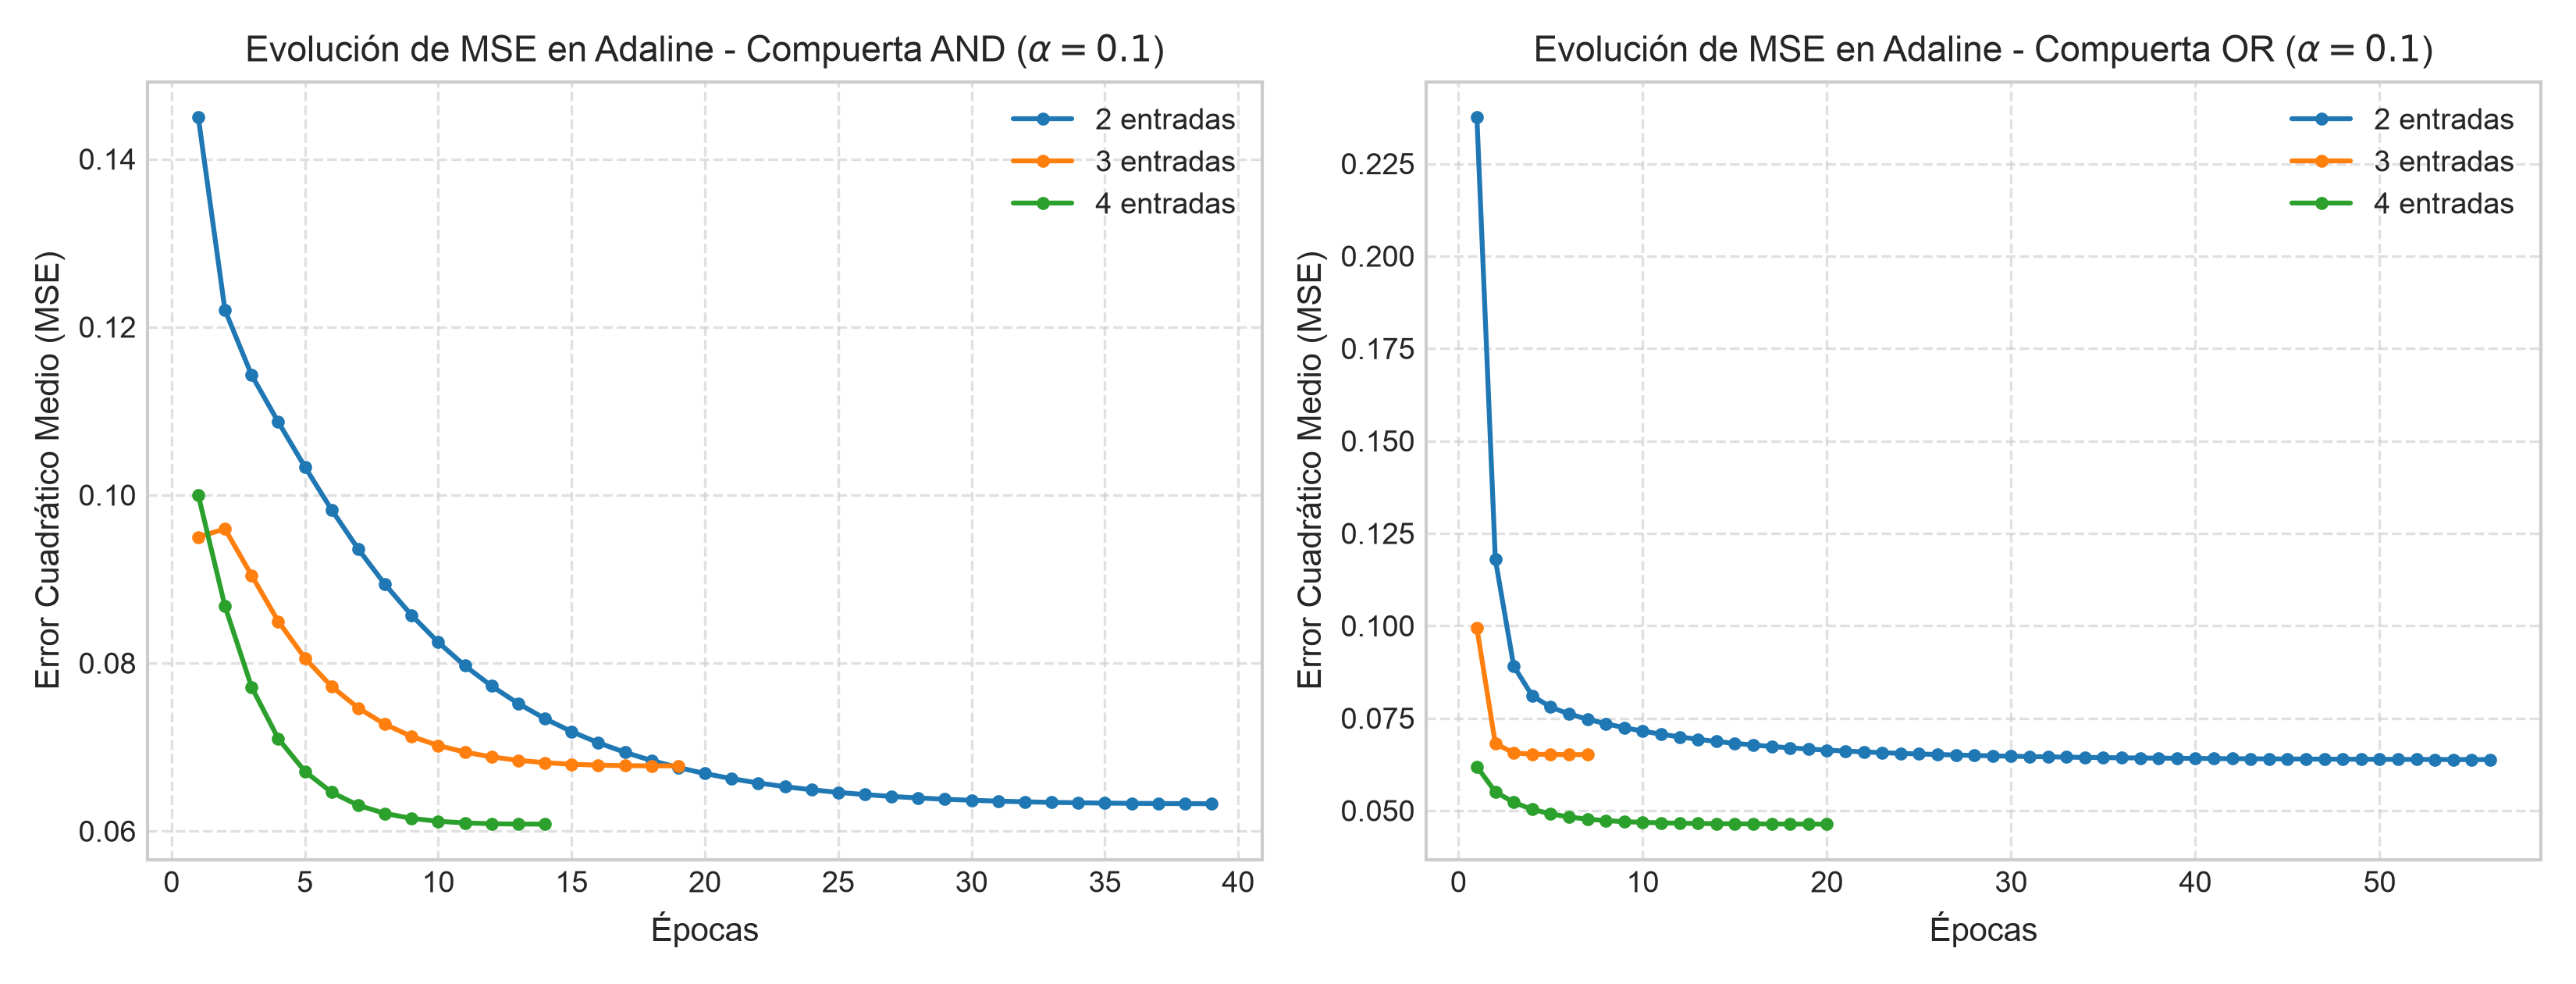
\includegraphics[width=0.88\textwidth]{figuras/compuertas_convergencia_adaline.png}
    \caption{Curvas de decaimiento del Error Cuadrático Medio (MSE) en Adaline para AND y OR ($\alpha = 0.1$).}
    \label{fig:compuertas_a}
\end{figure}

\subsection{Clasificación en Dataset Iris con Adaline (Punto 10)}
Las características continuas de Iris fueron estandarizadas. Se exploraron tasas $\alpha \in [0.001, 0.005, 0.01, 0.05, 0.1]$. Como resume la Tabla \ref{tab:iris_a} y la Figura \ref{fig:iris_a}, Adaline alcanza convergencia asintótica del MSE en menos de 50 épocas para $\alpha = 0.01$, logrando una exactitud de clasificación perfecta del \textbf{100.0\%} en todas las particiones.

\begin{table}[H]
\centering
\caption{Rendimiento de Adaline en Dataset Iris ($\alpha = 0.01$, $\theta = 0.5$).}
\label{tab:iris_a}
\begin{adjustbox}{max width=\textwidth}
\begin{tabular}{lcccccc}
\toprule
\textbf{Partición} & \textbf{Épocas} & \textbf{MSE Final} & \textbf{Exactitud Train} & \textbf{Exactitud Test} & \textbf{Vector de Pesos Final $[w_0, w_1, w_2, w_3, w_4]$} \\
\midrule
60-40 & 48 & 0.02333 & 100.0\% & 100.0\% & $[0.3397, 0.0366, 0.1334, -0.2721, -0.1182]$ \\
70-30 & 44 & 0.02182 & 100.0\% & 100.0\% & $[0.3343, 0.0231, 0.1332, -0.2813, -0.1168]$ \\
80-20 & 42 & 0.02183 & 100.0\% & 100.0\% & $[0.3326, 0.0240, 0.1106, -0.3162, -0.1046]$ \\
90-10 & 39 & 0.02080 & 100.0\% & 100.0\% & $[0.3371, 0.0171, 0.1064, -0.3165, -0.0983]$ \\
\bottomrule
\end{tabular}
\end{adjustbox}
\end{table}

\begin{figure}[H]
    \centering
    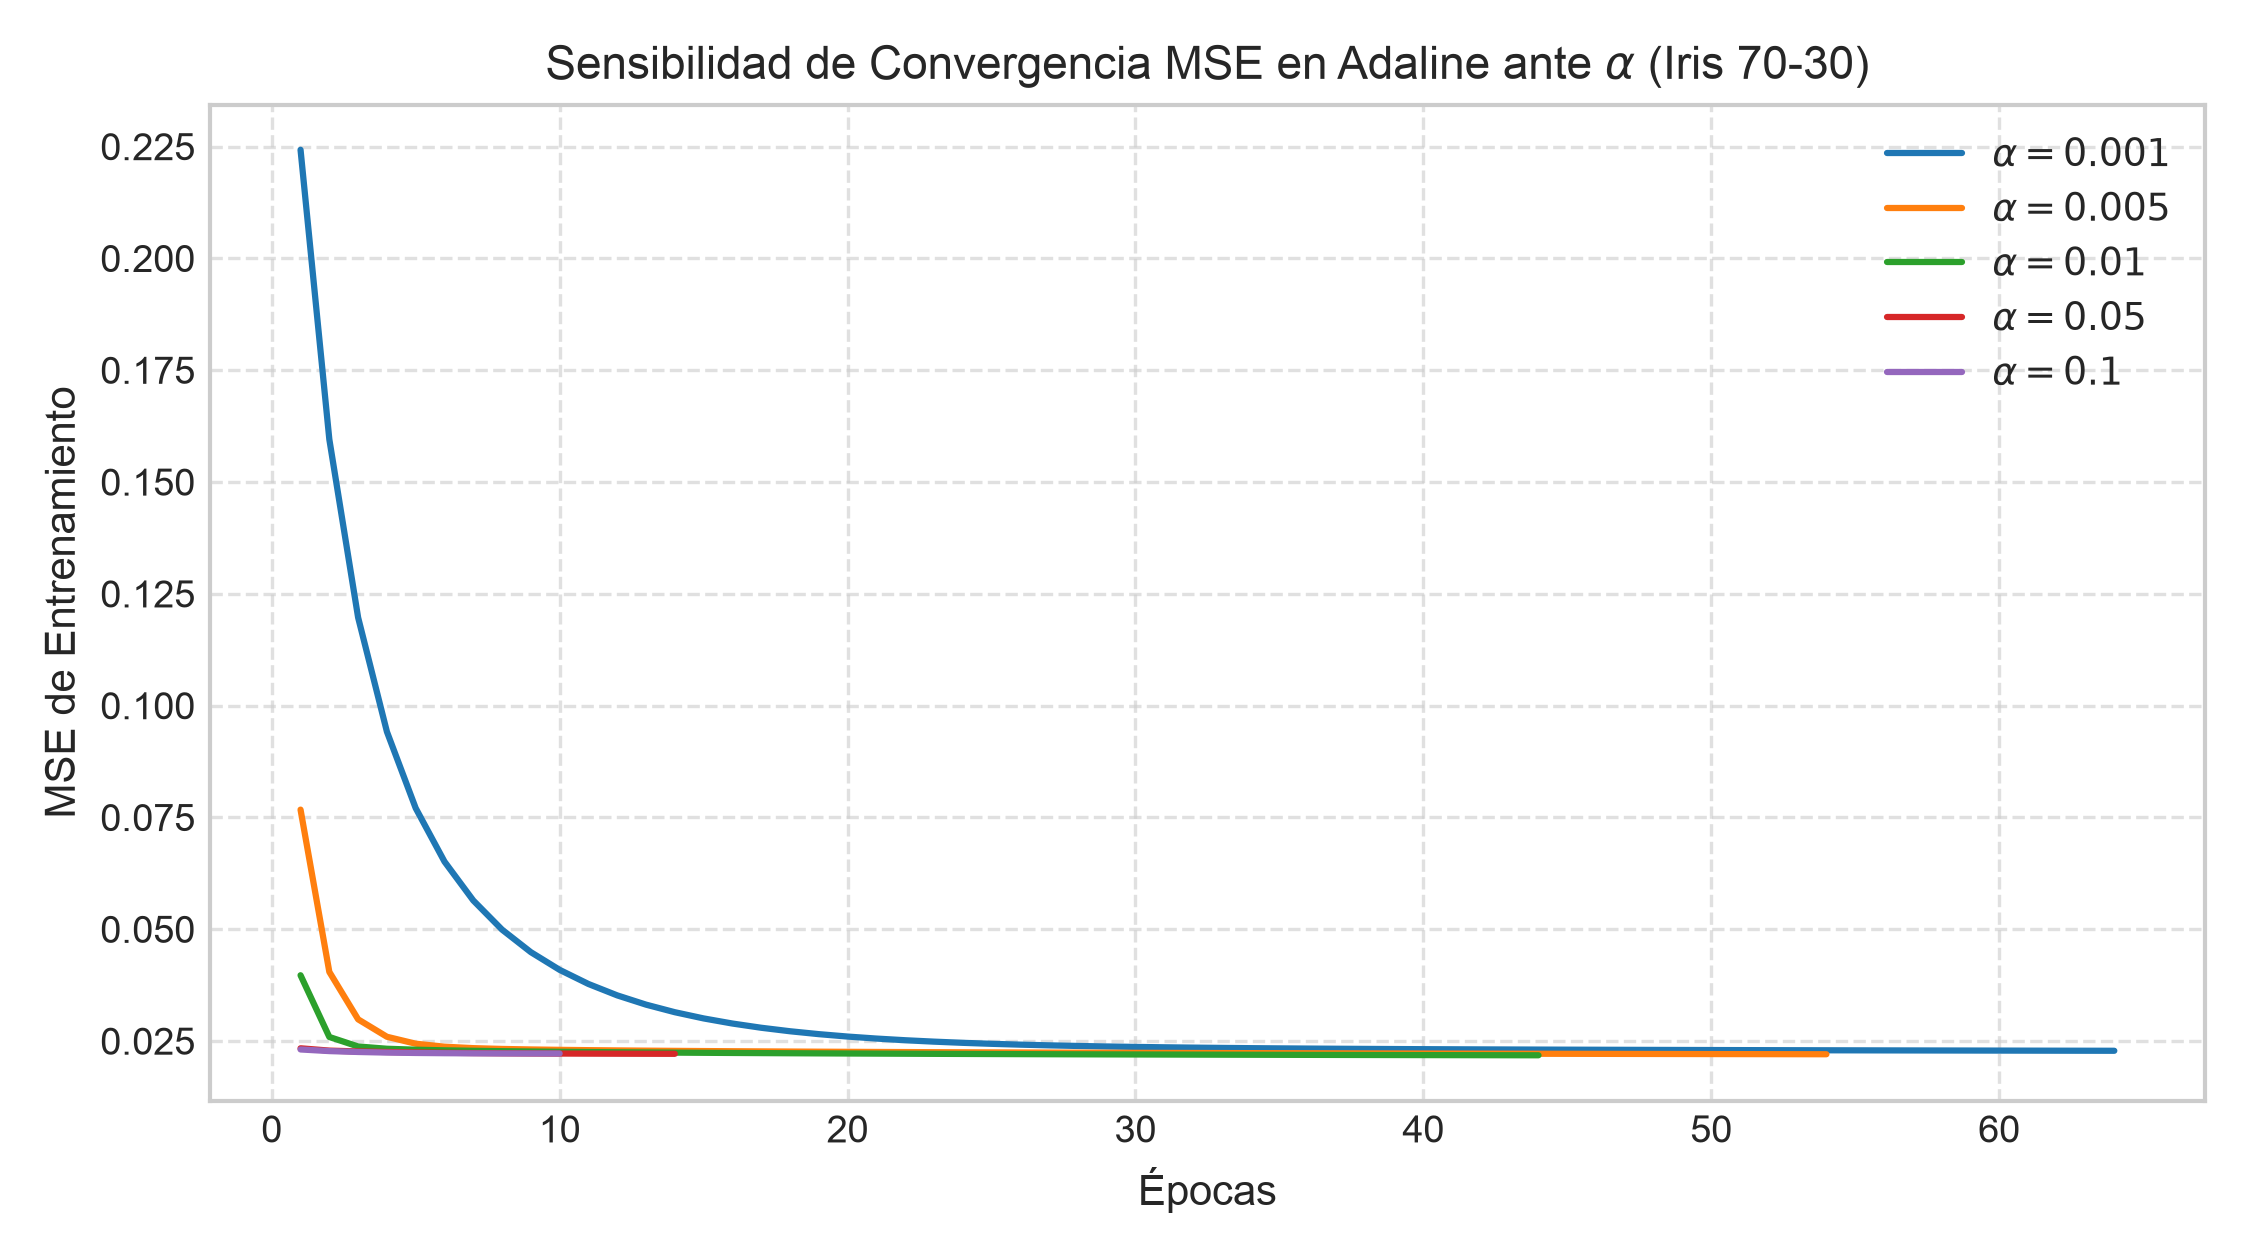
\includegraphics[width=0.65\textwidth]{figuras/iris_convergencia_adaline.png}
    \caption{Influencia de la tasa de aprendizaje $\alpha$ sobre la velocidad de decaimiento del MSE (Iris 70-30).}
    \label{fig:iris_a}
\end{figure}

\subsection{Clasificación en Banknote Authentication con Adaline (Puntos 11 y 12)}
En la Tabla \ref{tab:banknote_a} se presentan las métricas de prueba de Adaline bajo $\alpha = 0.005$. Se observa un MSE final estabilizado en $\approx 0.032$, con exactitudes de prueba entre el 96.5\% y el 97.1\%, y sensibilidades cercanas al 100\%.

\begin{table}[H]
\centering
\caption{Métricas de Adaline en Banknote Authentication ($\alpha = 0.005$, $\theta = 0.5$).}
\label{tab:banknote_a}
\begin{adjustbox}{max width=0.92\textwidth}
\begin{tabular}{lcccccc}
\toprule
\textbf{Partición} & \textbf{Épocas} & \textbf{MSE Final} & \textbf{Exactitud Test} & \textbf{Precisión} & \textbf{Sensibilidad} & \textbf{F1-Score} \\
\midrule
60-40 & 7 & 0.03177 & 96.54\% & 93.13\% & 99.59\% & 0.9625 \\
70-30 & 7 & 0.03260 & 96.84\% & 93.78\% & 99.45\% & 0.9653 \\
80-20 & 7 & 0.03277 & 97.09\% & 93.70\% & 100.0\% & 0.9675 \\
90-10 & 7 & 0.03320 & 97.10\% & 93.55\% & 100.0\% & 0.9667 \\
\bottomrule
\end{tabular}
\end{adjustbox}
\end{table}

\begin{figure}[H]
    \centering
    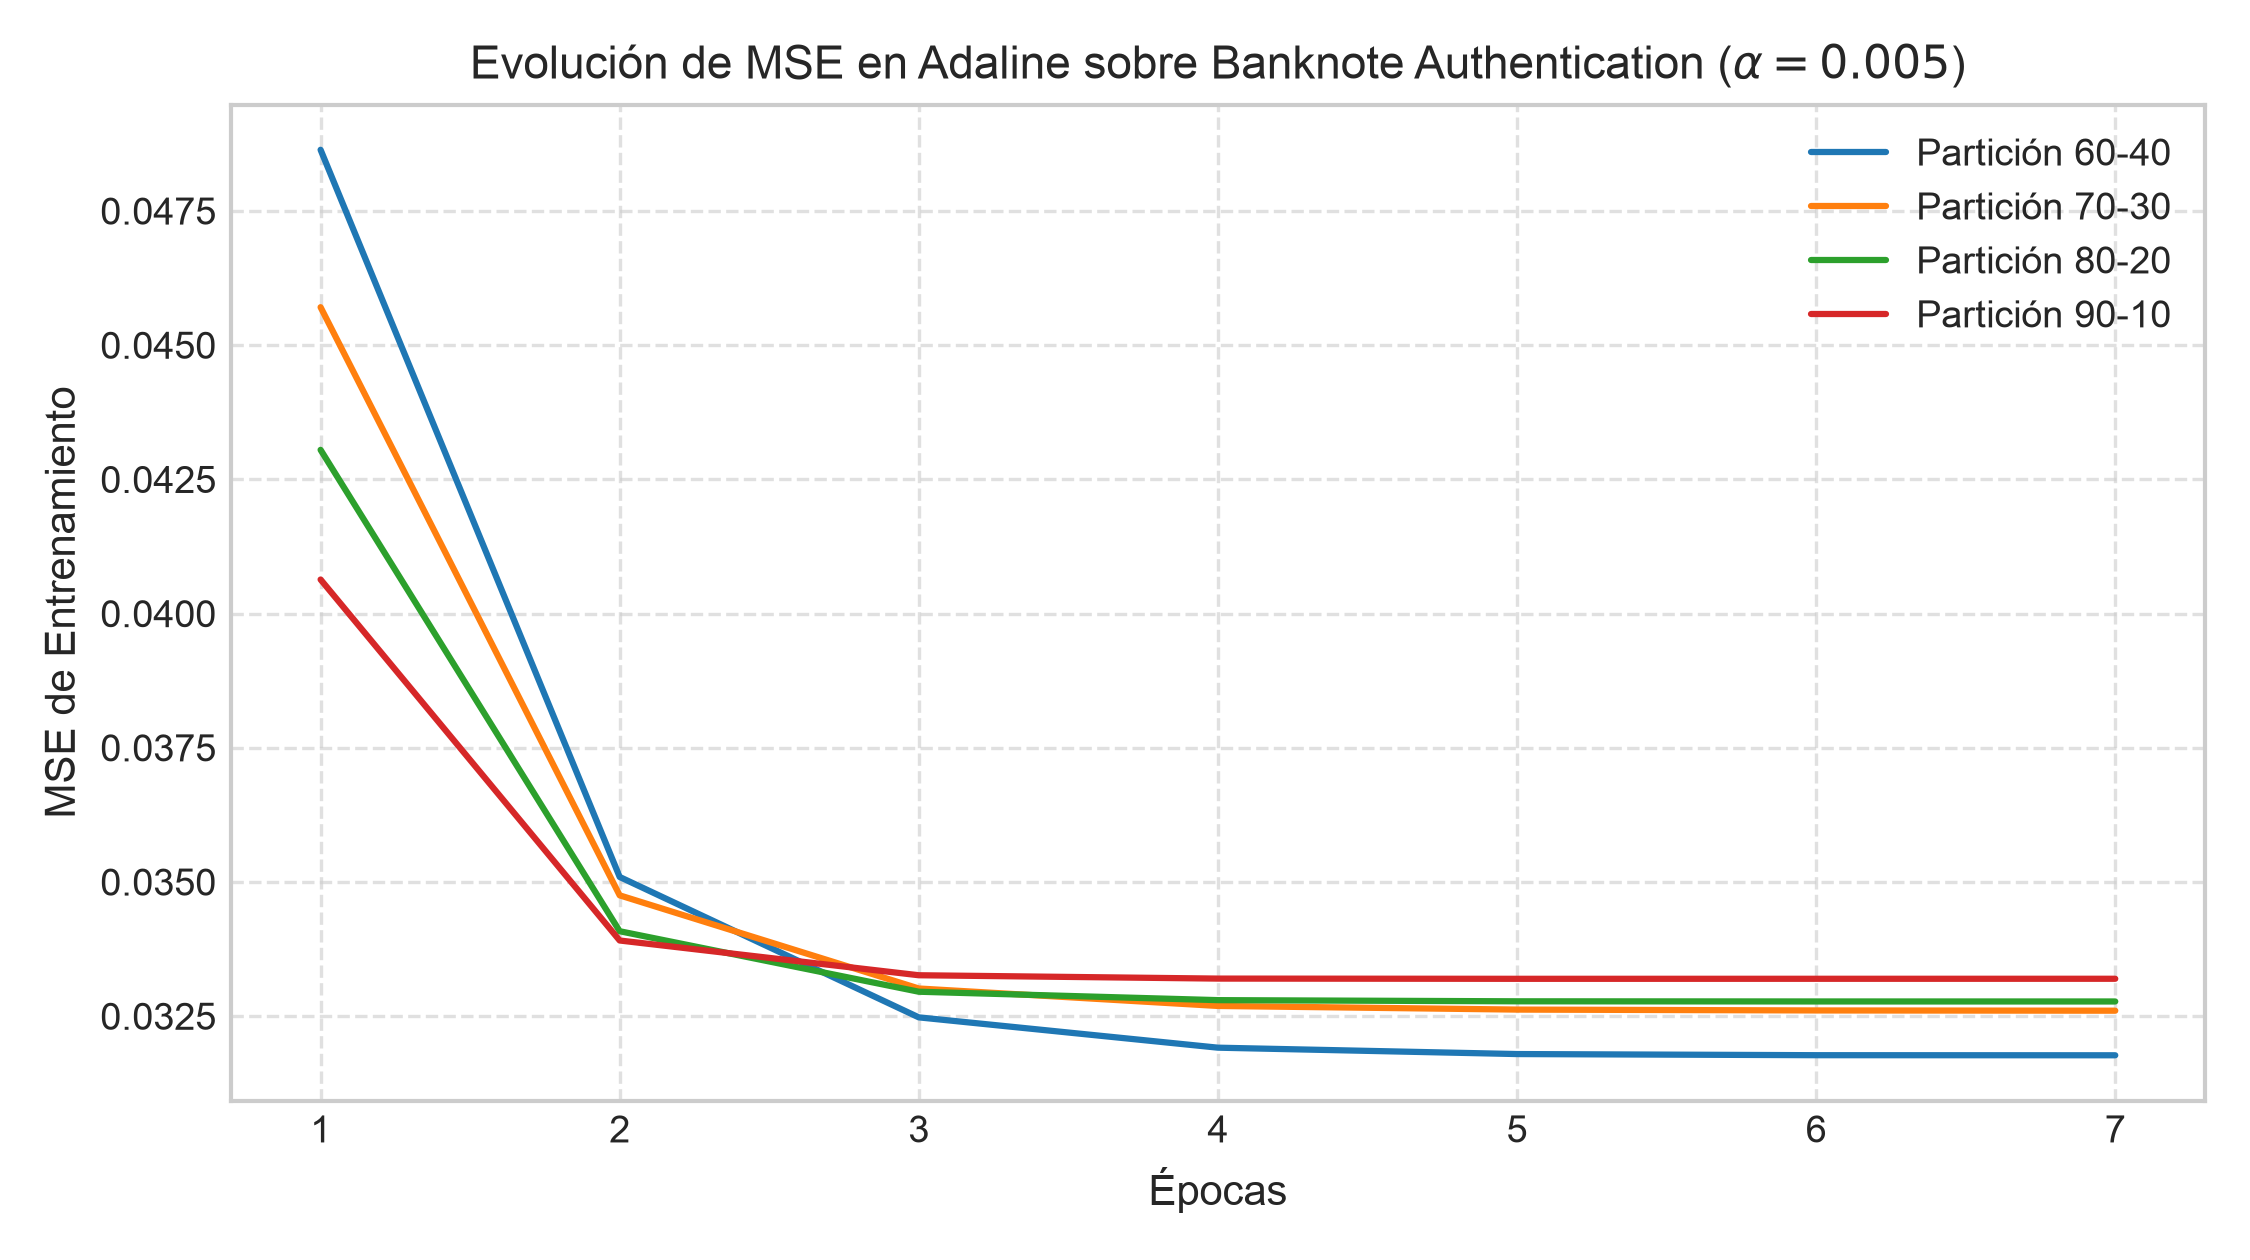
\includegraphics[width=0.65\textwidth]{figuras/banknote_convergencia_adaline.png}
    \caption{Convergencia del MSE en Adaline para Banknote Authentication bajo las 4 particiones.}
    \label{fig:banknote_a}
\end{figure}

% -------------------------------------------------------------
\section{Comparación Crítica: Perceptrón Simple vs Adaline}
En esta sección se sintetizan las diferencias conceptuales, cuantitativas y operacionales entre ambas arquitecturas neuronales.

\subsection{Fronteras de Decisión en el Espacio de Entradas}
La Figura \ref{fig:fronteras_2d} ilustra las fronteras de separación lineal inducidas en el plano cartesiano $[x_1, x_2]$ para las compuertas $\text{AND}$ y $\text{OR}$.
\begin{itemize}
    \item En el \textbf{Perceptrón}, el hiperplano se ubica en cualquier posición que satisfaga la separación estricta de las clases (cero errores discretos), deteniéndose inmediatamente tras clasificar la última muestra.
    \item En \textbf{Adaline}, la frontera lineal busca maximizar el ajuste de mínimos cuadrados con respecto a los valores diana continuos ($0$ y $1$), produciendo una frontera más centrada respecto a la distribución geométrica de los datos.
\end{itemize}

\begin{figure}[H]
    \centering
    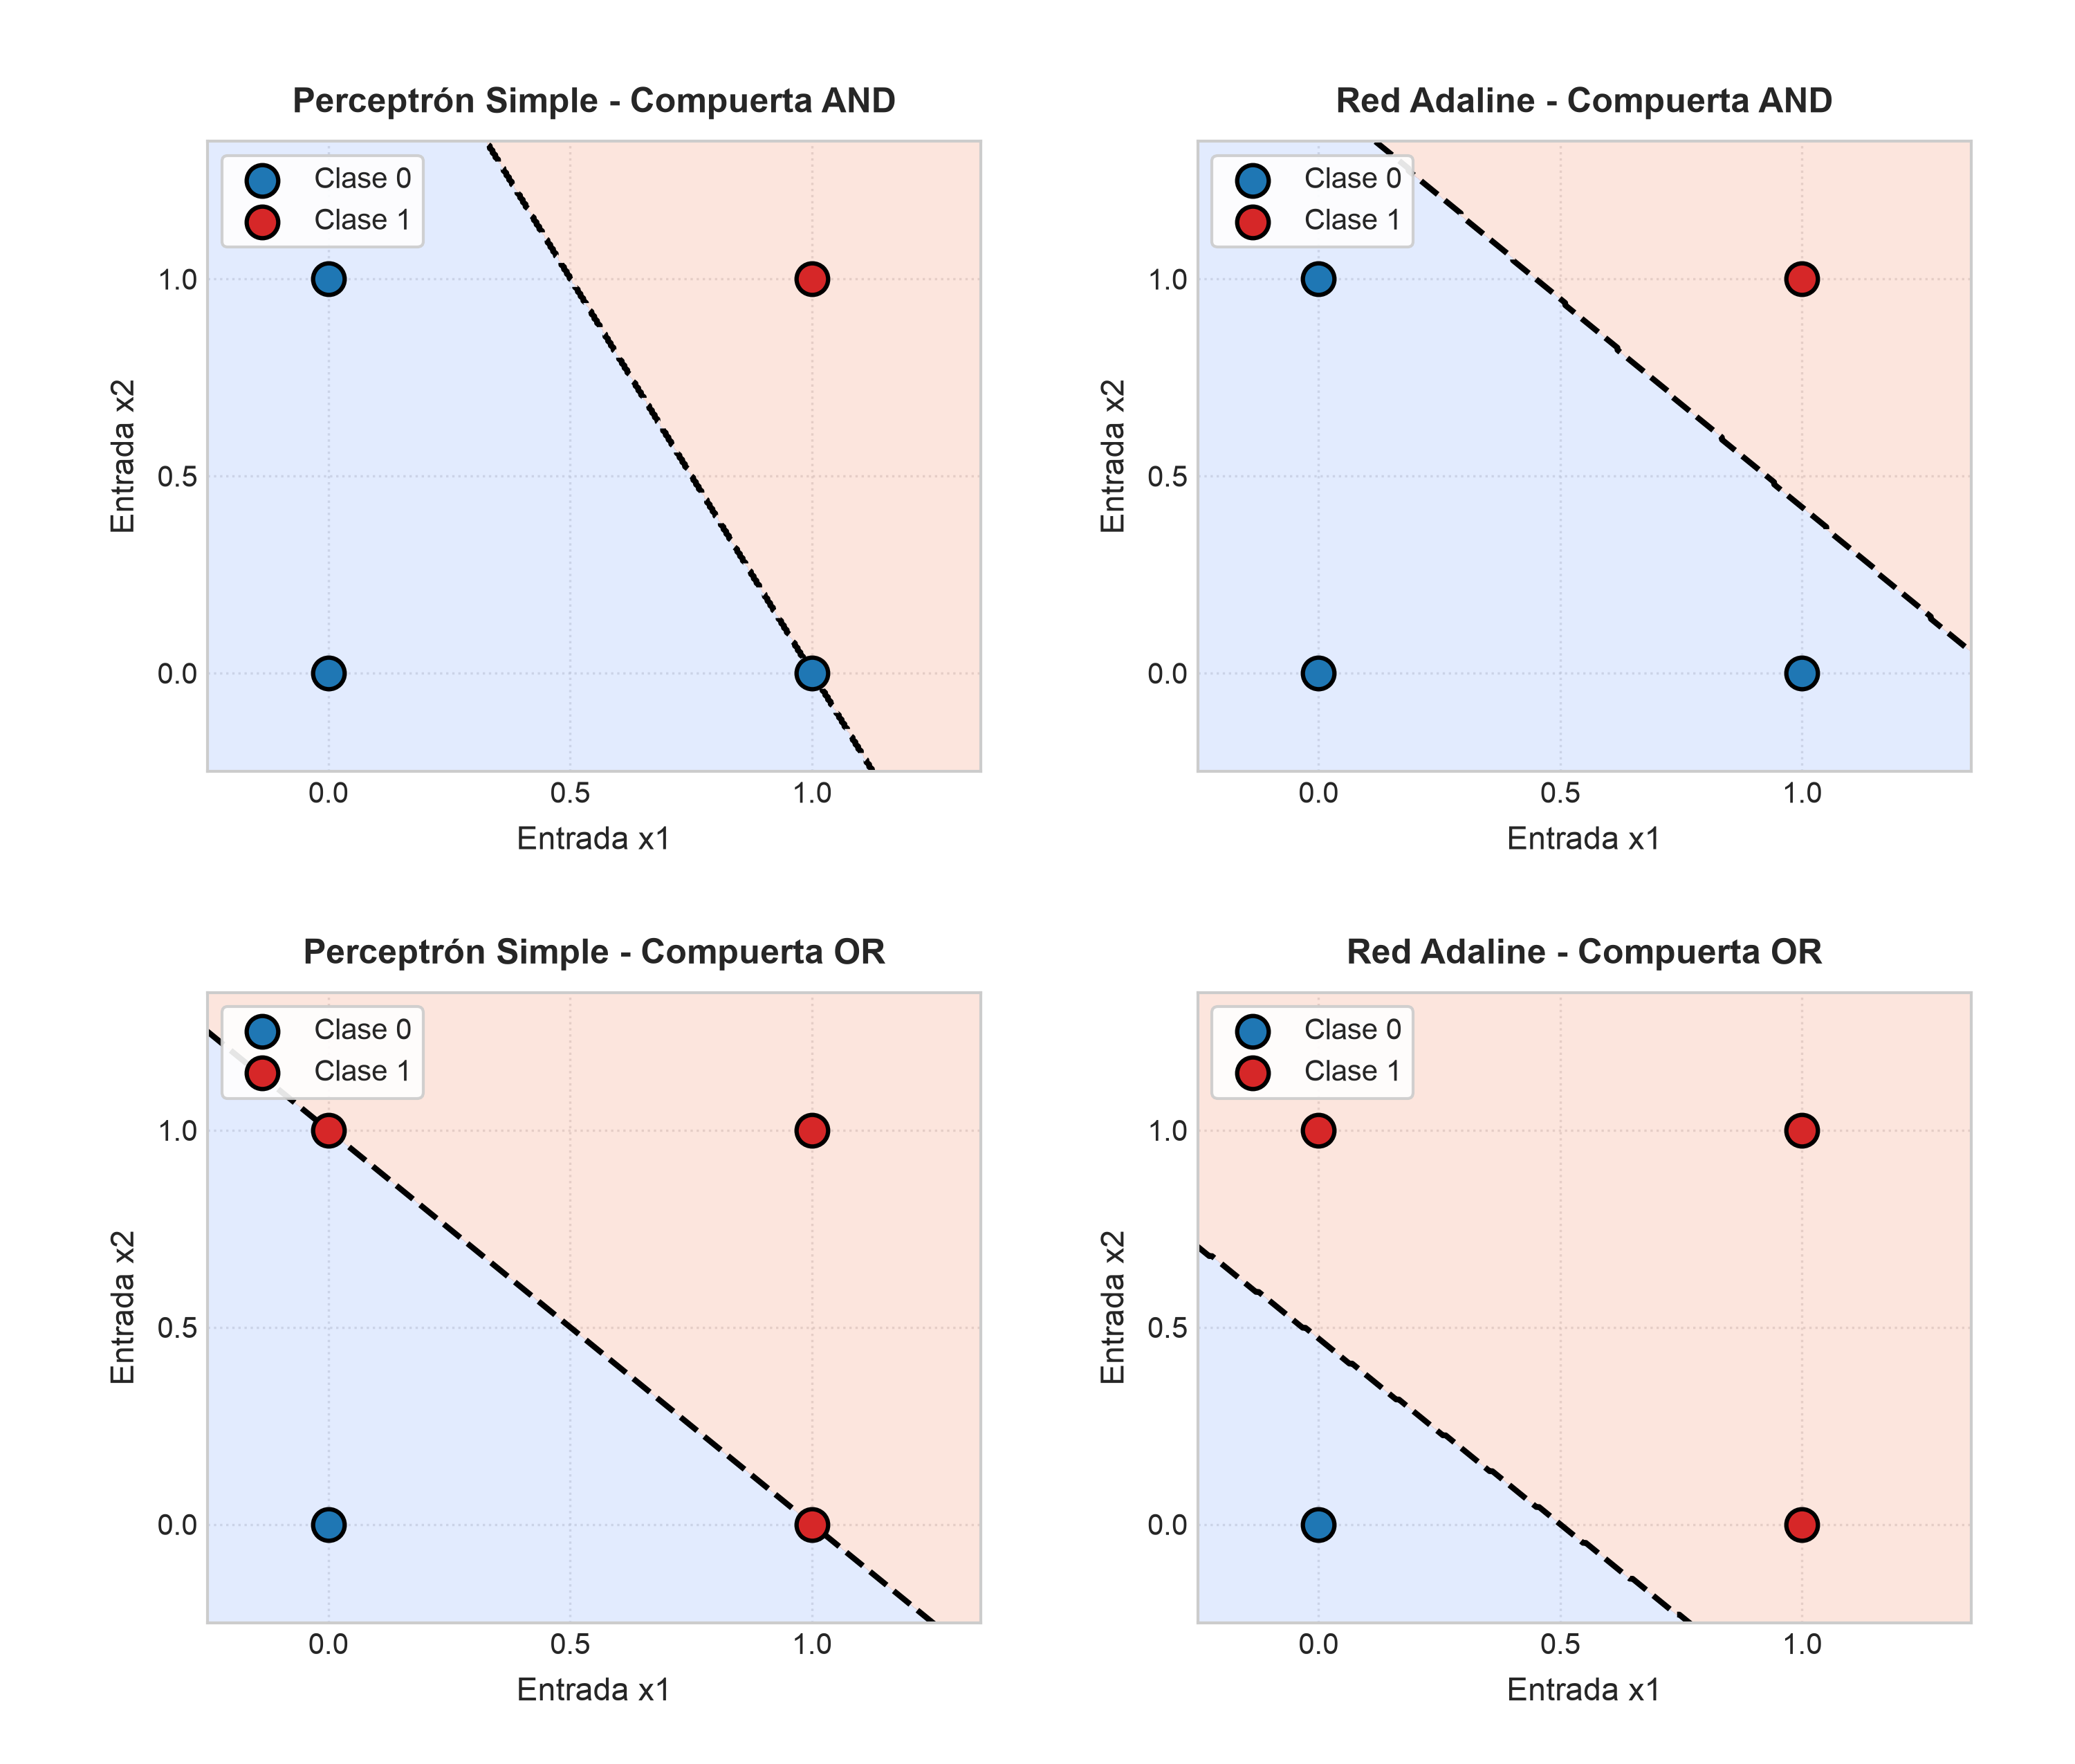
\includegraphics[width=0.88\textwidth]{figuras/fronteras_compuertas_2d.png}
    \caption{Comparación espacial de las fronteras de decisión: Perceptrón Simple vs Adaline en 2D.}
    \label{fig:fronteras_2d}
\end{figure}

\clearpage

\subsection{Matrices de Confusión y Análisis de Error}
La Figura \ref{fig:cm_comp} compara las matrices de confusión generadas sobre el 30\% de prueba del dataset Banknote Authentication. Ambos modelos exhiben una tasa de falsos negativos extraordinariamente baja (sensibilidad del 97.2\% al 99.4\%), confirmando que las transformadas Wavelet permiten proyectar el problema en un espacio de características cuasi-lineal.

\begin{figure}[H]
    \centering
    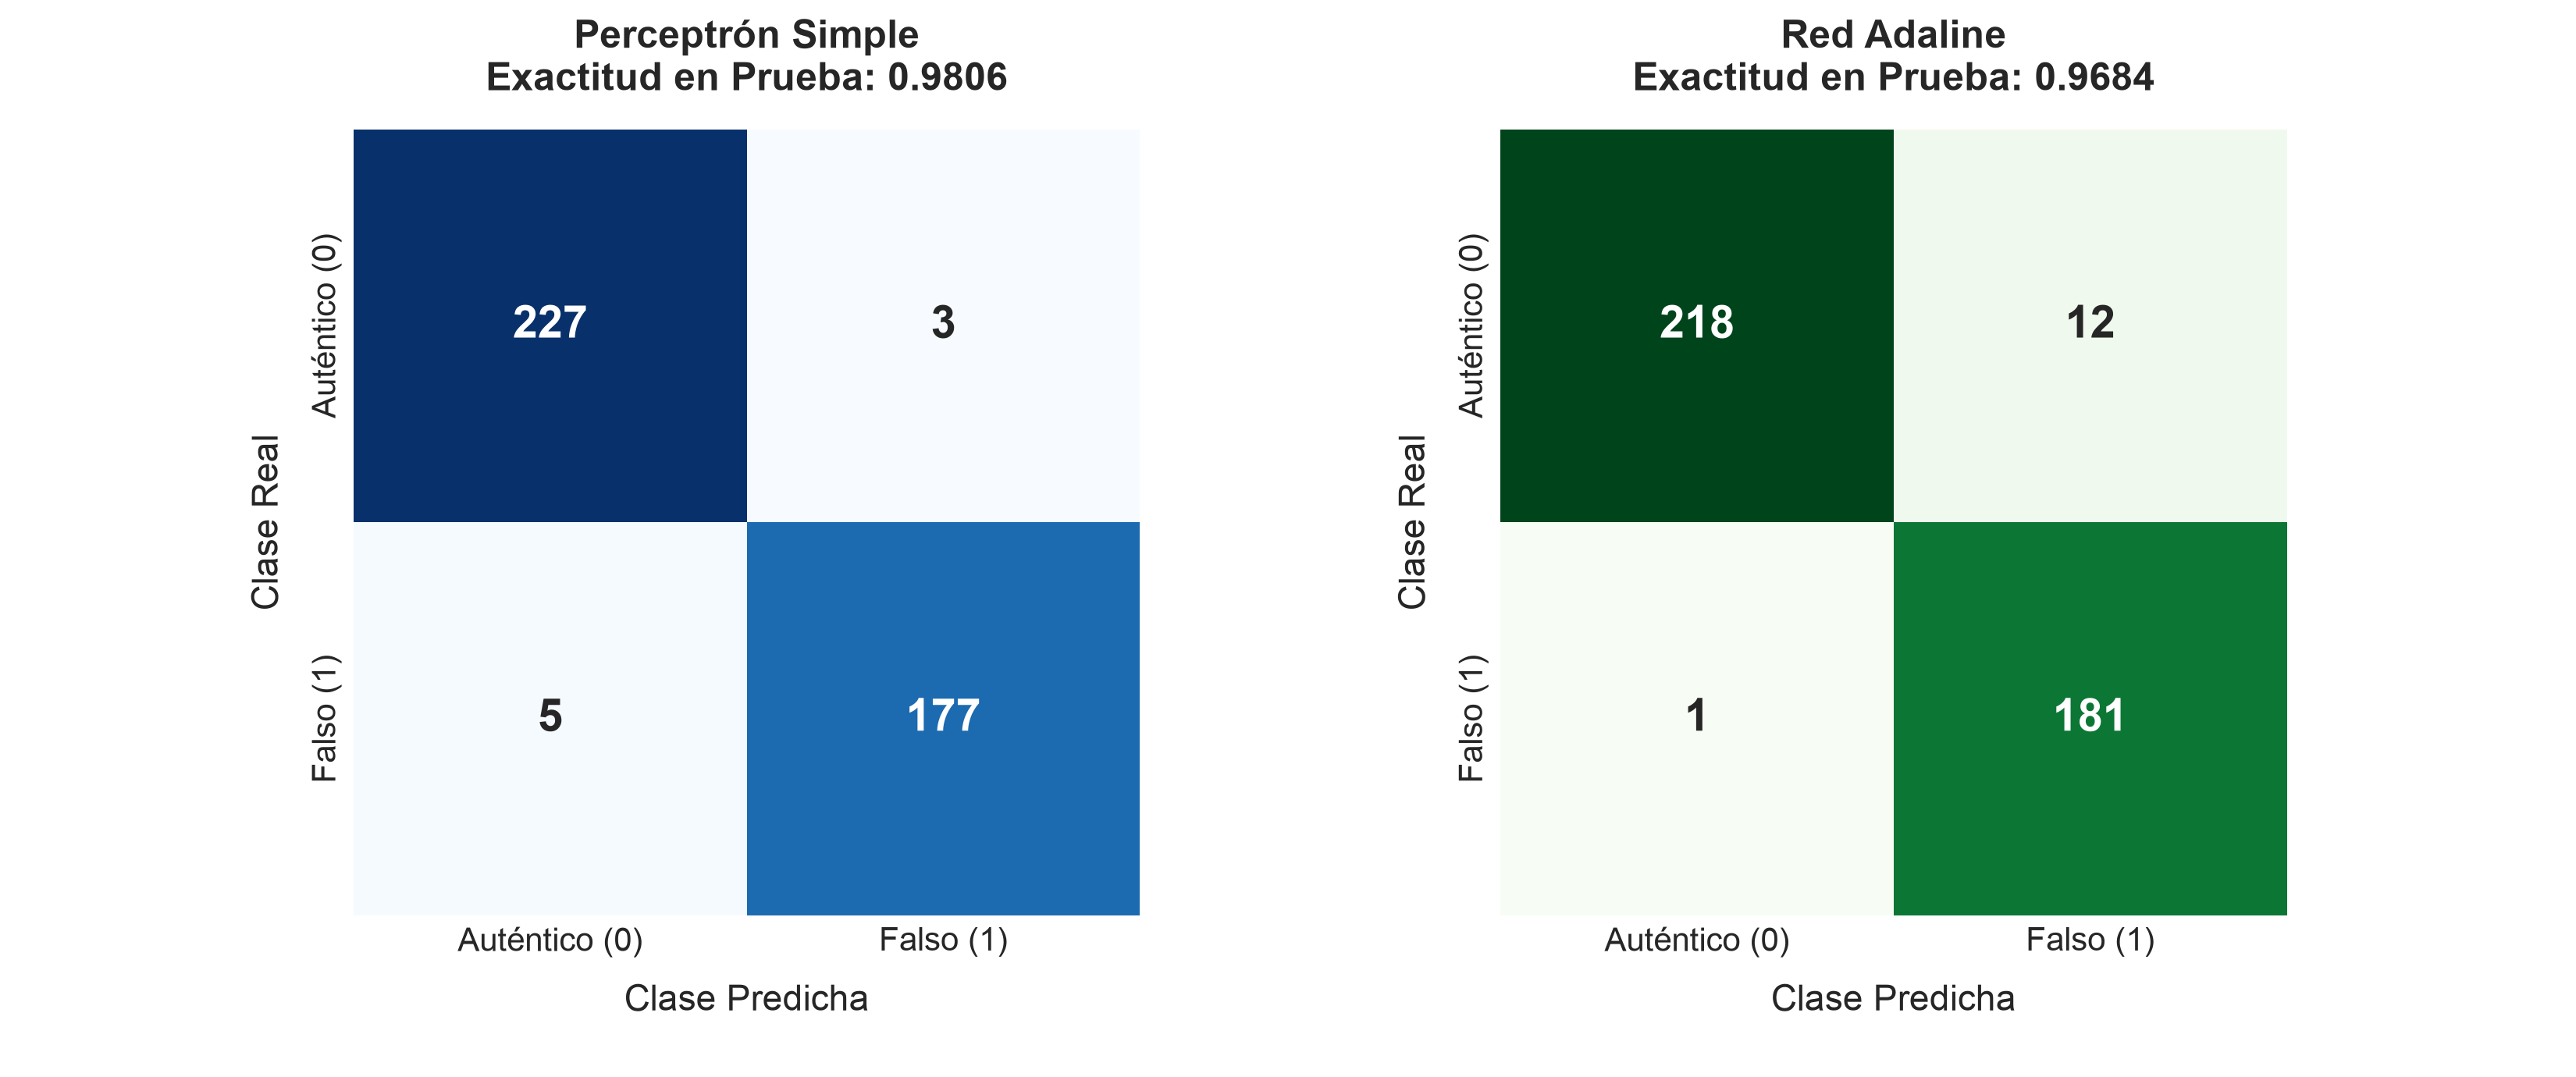
\includegraphics[width=0.88\textwidth]{figuras/matriz_confusion_comparativa.png}
    \caption{Matrices de confusión comparativas sobre el conjunto de prueba (Banknote 70-30).}
    \label{fig:cm_comp}
\end{figure}

\subsection{Rendimiento Global y Sensibilidad al Escalamiento}
La Figura \ref{fig:barras_comp} y la Tabla \ref{tab:cuadro_comparativo} resumen las diferencias operacionales fundamentales entre ambos modelos. Para la Tabla \ref{tab:cuadro_comparativo}, se empleó el entorno \texttt{tabularx} con el objetivo de garantizar ajuste perfecto al ancho del texto y ajuste automático de párrafos en cada celda.

\begin{figure}[H]
    \centering
    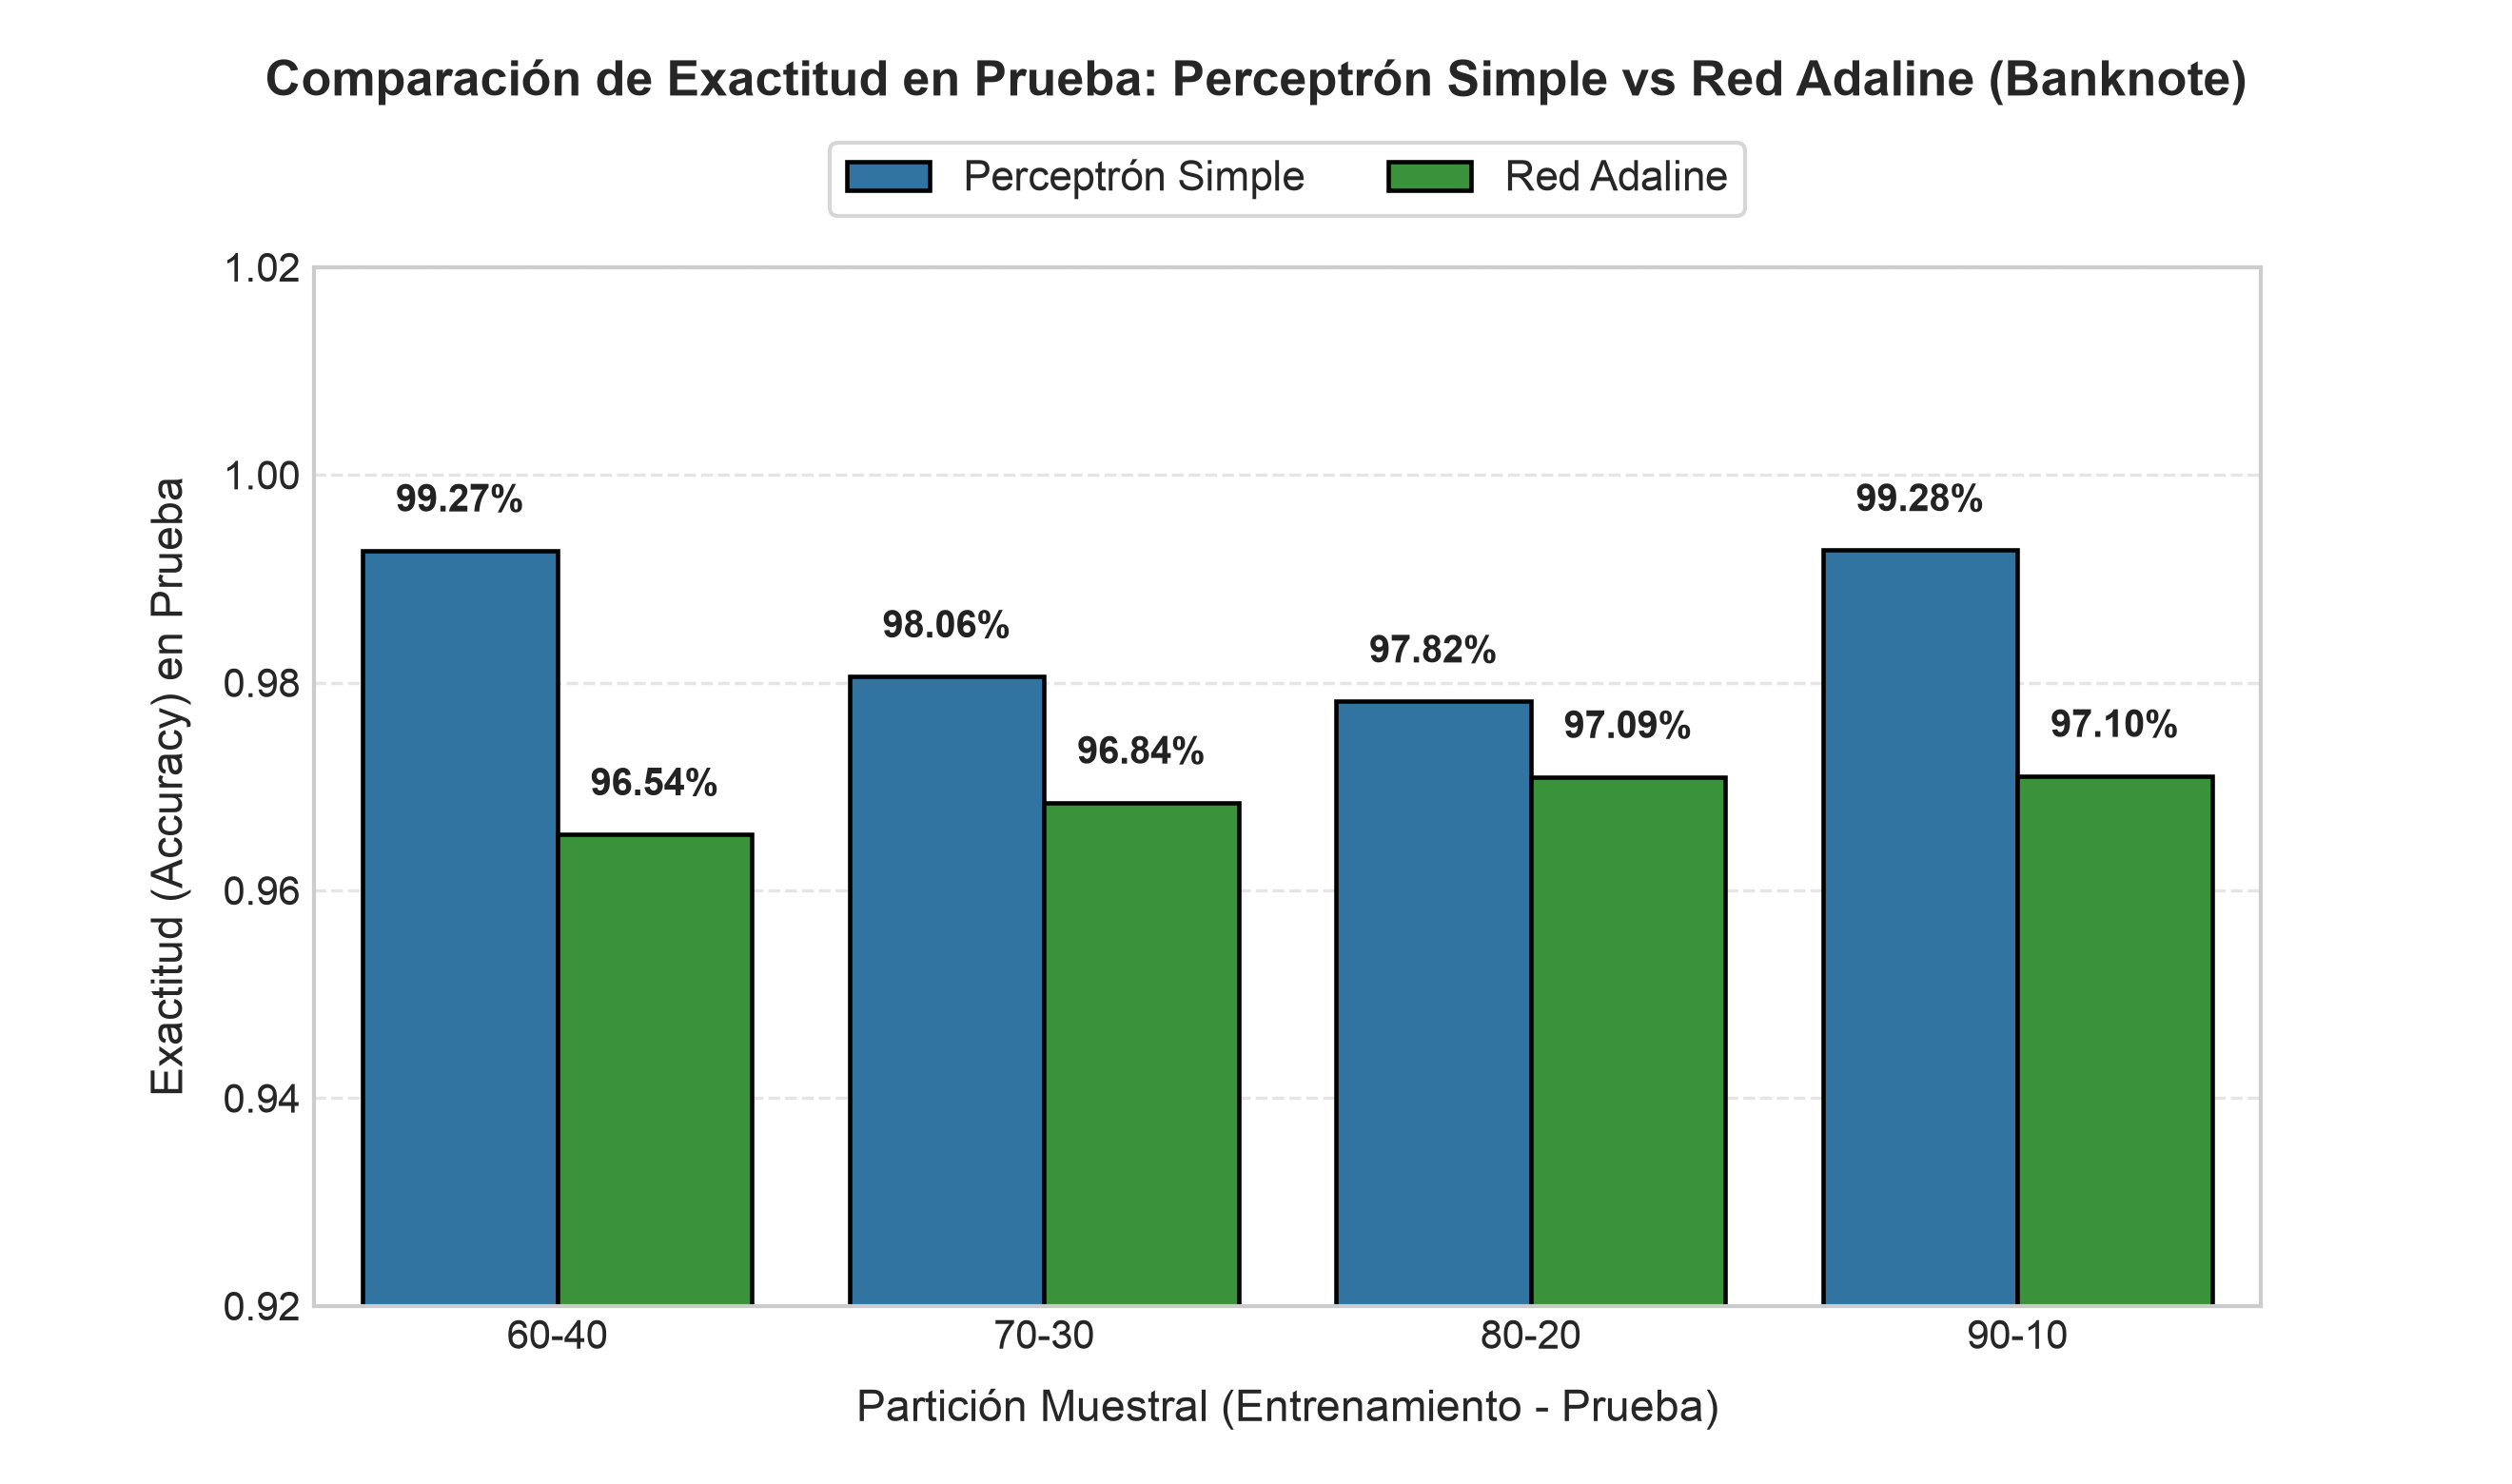
\includegraphics[width=0.75\textwidth]{figuras/comparacion_perceptron_adaline.png}
    \caption{Exactitud en prueba según la partición de datos: Perceptrón Simple vs Adaline.}
    \label{fig:barras_comp}
\end{figure}

\clearpage

\begin{table}[H]
\centering
\caption{Cuadro comparativo multidimensional entre el Perceptrón Simple y la Red Adaline.}
\label{tab:cuadro_comparativo}
\begin{tabularx}{\textwidth}{p{3.3cm} X X}
\toprule
\textbf{Criterio Evaluado} & \textbf{Perceptrón Simple (Rosenblatt)} & \textbf{Red Adaline (Widrow-Hoff)} \\
\midrule
\textbf{Función de Activación} & Escalón Unitario (Discreta, Heaviside). Produce salidas binarias $\{0, 1\}$. & Lineal $Y(x) = W^T X$ continua en entrenamiento; umbral $\theta$ en inferencia. \\
\addlinespace
\textbf{Cálculo del Error} & Posterior al umbral: $e = d(x) - Y_{disc}$. Cuantizado en $\{-1, 0, +1\}$. & Previo al umbral: $e = d(x) - Y_{lineal}$. Magnitud continua suave. \\
\addlinespace
\textbf{Criterio de Optimización} & Corrección heurística por error de clasificación discreto. & Descenso de gradiente estocástico sobre la superficie analítica de mínimos cuadrados. \\
\addlinespace
\textbf{Función de Costo} & No diferenciable, con gradiente nulo en casi todo punto (escalón). & Cuadrática convexa (MSE). Posee un único mínimo global garantizado. \\
\addlinespace
\textbf{Garantía de Convergencia} & Teorema de Rosenblatt: converge en número finito de pasos si el conjunto es linealmente separable. & Converge asintóticamente al mínimo de MSE para cualquier tasa $\alpha$ dentro del radio espectral. \\
\addlinespace
\textbf{Sensibilidad a la Escala} & Moderada: la magnitud de las entradas influye en la tasa efectiva de giro del plano. & Muy alta: gradientes no escalados provocan divergencias numéricas severas. Requiere estandarización. \\
\addlinespace
\textbf{Rendimiento en Banknote} & Exactitud de prueba: $\approx 98.1\% - 99.3\%$. F1-Score: $> 0.975$. & Exactitud de prueba: $\approx 96.5\% - 97.1\%$. Sensibilidad: hasta $100.0\%$. \\
\bottomrule
\end{tabularx}
\end{table}

% -------------------------------------------------------------
\section{Conclusiones}
El problema central que revelan estos experimentos no es escoger entre el Perceptrón y Adaline como si uno de ellos ofreciera una solución universal, sino establecer qué significa realmente que un modelo ``funcione''. La Regla 1, $\Delta W_i = d(x)X_i$, no constituye un mecanismo de aprendizaje discriminativo: al no incorporar la predicción ni el signo del error, carece de una respuesta correctiva ante los falsos positivos y empuja los pesos en una sola dirección; su deterioro en las compuertas AND no es una anomalía experimental, sino la consecuencia necesaria de una regla incapaz de representar el conflicto entre clases. Las Reglas 2 y 3 corrigen esta deficiencia, pero la convergencia del Perceptrón solo tiene significado cuando existe separabilidad lineal y depende de la escala de las variables, del orden de presentación y de $\alpha$; por tanto, alcanzar cero errores en Iris o en las compuertas no demuestra robustez general, sino que confirma que esos conjuntos permiten una frontera lineal bajo las condiciones ensayadas. Adaline expone una limitación distinta: minimizar una función MSE convexa garantiza un ajuste continuo de los pesos, no una clasificación óptima. Sus resultados en Banknote muestran que una salida aparentemente estable puede conservar errores relevantes al aplicar el umbral $\theta = 0.5$, especialmente cuando la regresión lineal aproxima etiquetas binarias y las clases no quedan simétricamente distribuidas. En consecuencia, el escalamiento, la elección de $\alpha$, el umbral y la partición de los datos no son detalles operativos, sino parte del resultado y de su validez; incluso las exactitudes superiores al 97\% deben leerse como evidencia condicionada al protocolo utilizado, no como una propiedad intrínseca de los modelos. La conclusión más exigente es, entonces, que estas arquitecturas son útiles precisamente porque hacen visibles sus supuestos: una regla de actualización sin retroalimentación fracasa por construcción, una frontera lineal no resuelve problemas no separables y una métrica de optimización no equivale al objetivo de clasificación. El valor del análisis está en delimitar esas condiciones y evitar que una convergencia rápida o un porcentaje alto de exactitud se confundan con capacidad predictiva generalizable.

% -------------------------------------------------------------
\section{Referencias Bibliográficas}
\begin{enumerate}
    \item F. Rosenblatt, ``The Perceptron: A probabilistic model for information storage and organization in the brain,'' \textit{Psychological Review}, vol. 65, no. 6, pp. 386--408, 1958.
    \item B. Widrow and M. E. Hoff, ``Adaptive switching circuits,'' in \textit{IRE WESCON Convention Record}, part 4, pp. 96--104, 1960.
    \item S. Haykin, \textit{Neural Networks and Learning Machines}, 3rd ed. Upper Saddle River, NJ: Pearson Prentice Hall, 2009.
    \item S. Raschka and V. Mirjalili, \textit{Python Machine Learning: Machine Learning and Deep Learning with Python, scikit-learn, and TensorFlow 2}, 3rd ed. Birmingham: Packt Publishing, 2019.
    \item Dua, D. and Graff, C., ``UCI Machine Learning Repository: Banknote Authentication Dataset,'' School of Information and Computer Science, University of California, Irvine, 2017.
\end{enumerate}

\end{document}
